%Copyright 2019 Christopher M. Jermaine (cmj4@rice.edu) and Risa B. Myers (rbm2@rice.edu)
%
%Licensed under the Apache License, Version 2.0 (the "License");
%you may not use this file except in compliance with the License.
%You may obtain a copy of the License at
%
%    https://www.apache.org/licenses/LICENSE-2.0
%
%Unless required by applicable law or agreed to in writing, software
%distributed under the License is distributed on an "AS IS" BASIS,
%WITHOUT WARRANTIES OR CONDITIONS OF ANY KIND, either express or implied.
%See the License for the specific language governing permissions and
%limitations under the License.
%===============================================================
 \documentclass[aspectratio=169]{beamer}
\mode<presentation>
{
\usetheme[noshadow, minimal,numbers,riceb,nonav]{Rice}
\usefonttheme[onlymath]{serif}
\setbeamercovered{transparent}
}
\useinnertheme{rectangles}

\usepackage[english]{babel}

\usepackage{mathptmx}
\usepackage{helvet}
\usepackage{courier}
\usepackage[T1]{fontenc}
\usepackage{trajan}
\usepackage{ textcomp }
\usepackage{listings}

\newenvironment{noindentitemize}
{ \begin{itemize}
 \setlength{\itemsep}{1.5ex}
  \setlength{\parsep}{0pt}   
  \setlength{\parskip}{0pt}
 \addtolength{\leftskip}{-2em}
 }
{ \end{itemize} }

\newenvironment{noindentitemize2}
{ \begin{itemize}
  \setlength{\itemsep}{0ex}
  \setlength{\parskip}{0pt}
  \setlength{\parsep}{0pt}   
  \addtolength{\leftskip}{-2em}  }
{ \end{itemize} }

\lstnewenvironment{SQL}
  {\lstset{
        aboveskip=5pt,
        belowskip=5pt,
        escapechar=!,
        mathescape=true,
        upquote=true,
        language=SQL,
        basicstyle=\linespread{0.94}\ttfamily\footnotesize,
        morekeywords={WHILE, DO, END},
        deletekeywords={VALUE, PRIOR},
        showstringspaces=true}
        \vspace{0pt}%
        \noindent\minipage{0.47\textwidth}}
  {\endminipage\vspace{0pt}}
  
\newcommand{\LIKES}{\textrm{LIKES}} 
\newcommand{\FREQUENTS}{\textrm{FREQUENTS}} 
\newcommand{\SERVES}{\textrm{SERVES}} 
\newcommand{\CAFE}{\textrm{CAFE}} 
\newcommand{\COFFEE}{\textrm{COFFEE}} 
\newcommand{\DRINKER}{\textrm{DRINKER}} 
\newcommand{\ALLPEEPS}{\textrm{ALLPEEPS}} 
\newcommand{\ALLCOMBOS}{\textrm{ALLCOMBOS}} 


\setbeamerfont{block body}{size=\tiny}

%===============================================================%

\title[]
{Tools \& Models for Data Science}

\subtitle{Introduction to Unsupervised Learning}

\author[]{Chris Jermaine \& Risa Myers}
\institute
{
  Rice University 
}

\date[]{}

\subject{Beamer}

\begin{document}

\begin{frame}
 \titlepage
\end{frame}


%***********************************************************
\begin{frame}{Learning From Unlabeled Data}

\begin{columns}[T]
\begin{column}{0.5\textwidth}
    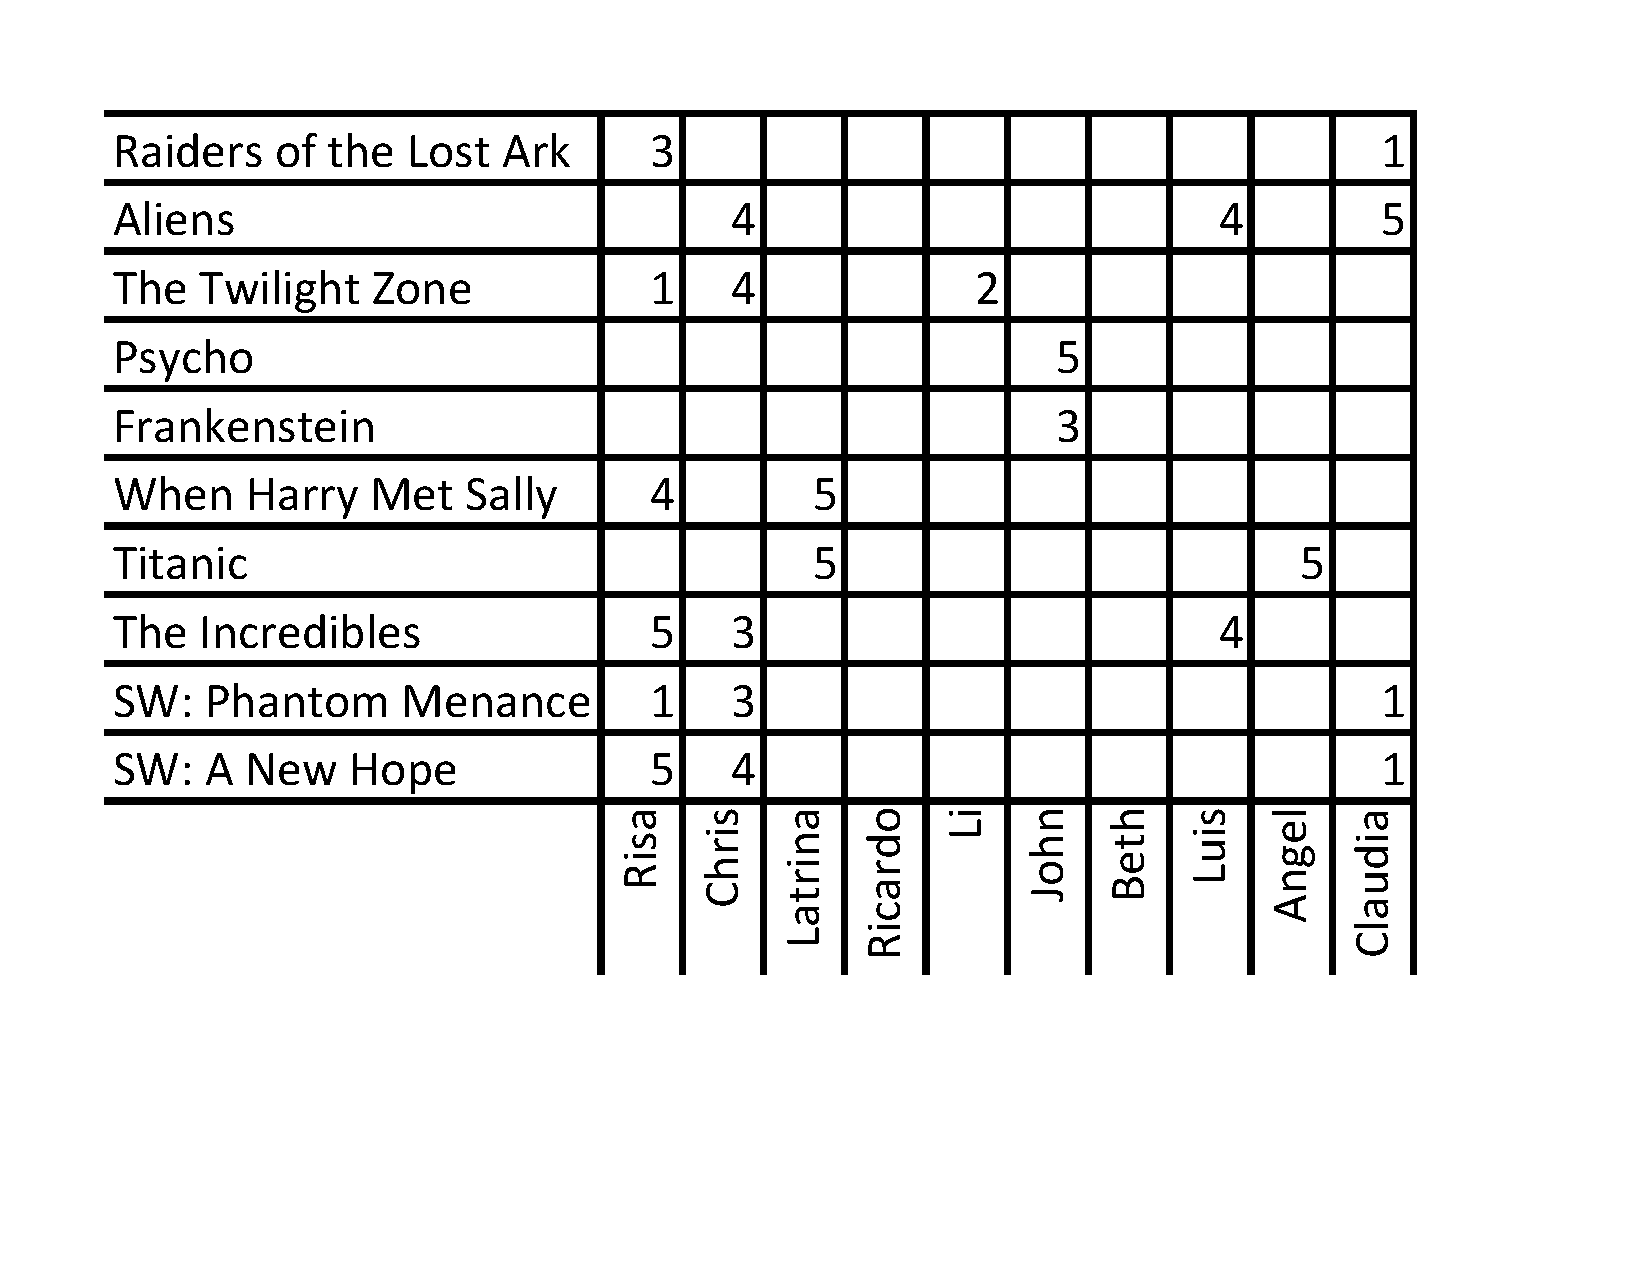
\includegraphics[width=1\textwidth]{lectUL/movieGrid} 
\end{column}
\begin{column}{0.5\textwidth}
\begin{itemize}
	\item Sometimes you have a data set without labels
        \begin{itemize}
                \item (height, weight, age, shoe size) quadruples for this class
		\item Register transactions from Wal-Mart
		\item User-Movie rating matrix 
        \end{itemize}
\end{itemize}
\end{column}
\end{columns}

\end{frame}%***********************************************************
\begin{frame}{Learning From Unlabeled Data}

\begin{columns}
\begin{column}{0.5\textwidth}
\begin{itemize}
	\item The goal is explanatory: 
        \begin{itemize}
		\item What to learn a model to help ``understand'' the data, in some sense
		\item Goal is not to predict some value(s) (though that might be a by-product)
		\item Movie Example
		        \begin{itemize}
			\item Group movies together
			\item Group viewer together
			\item Identify types of movies
        			\end{itemize}
        \end{itemize}
\end{itemize}
\end{column}
\begin{column}{0.5\textwidth}
    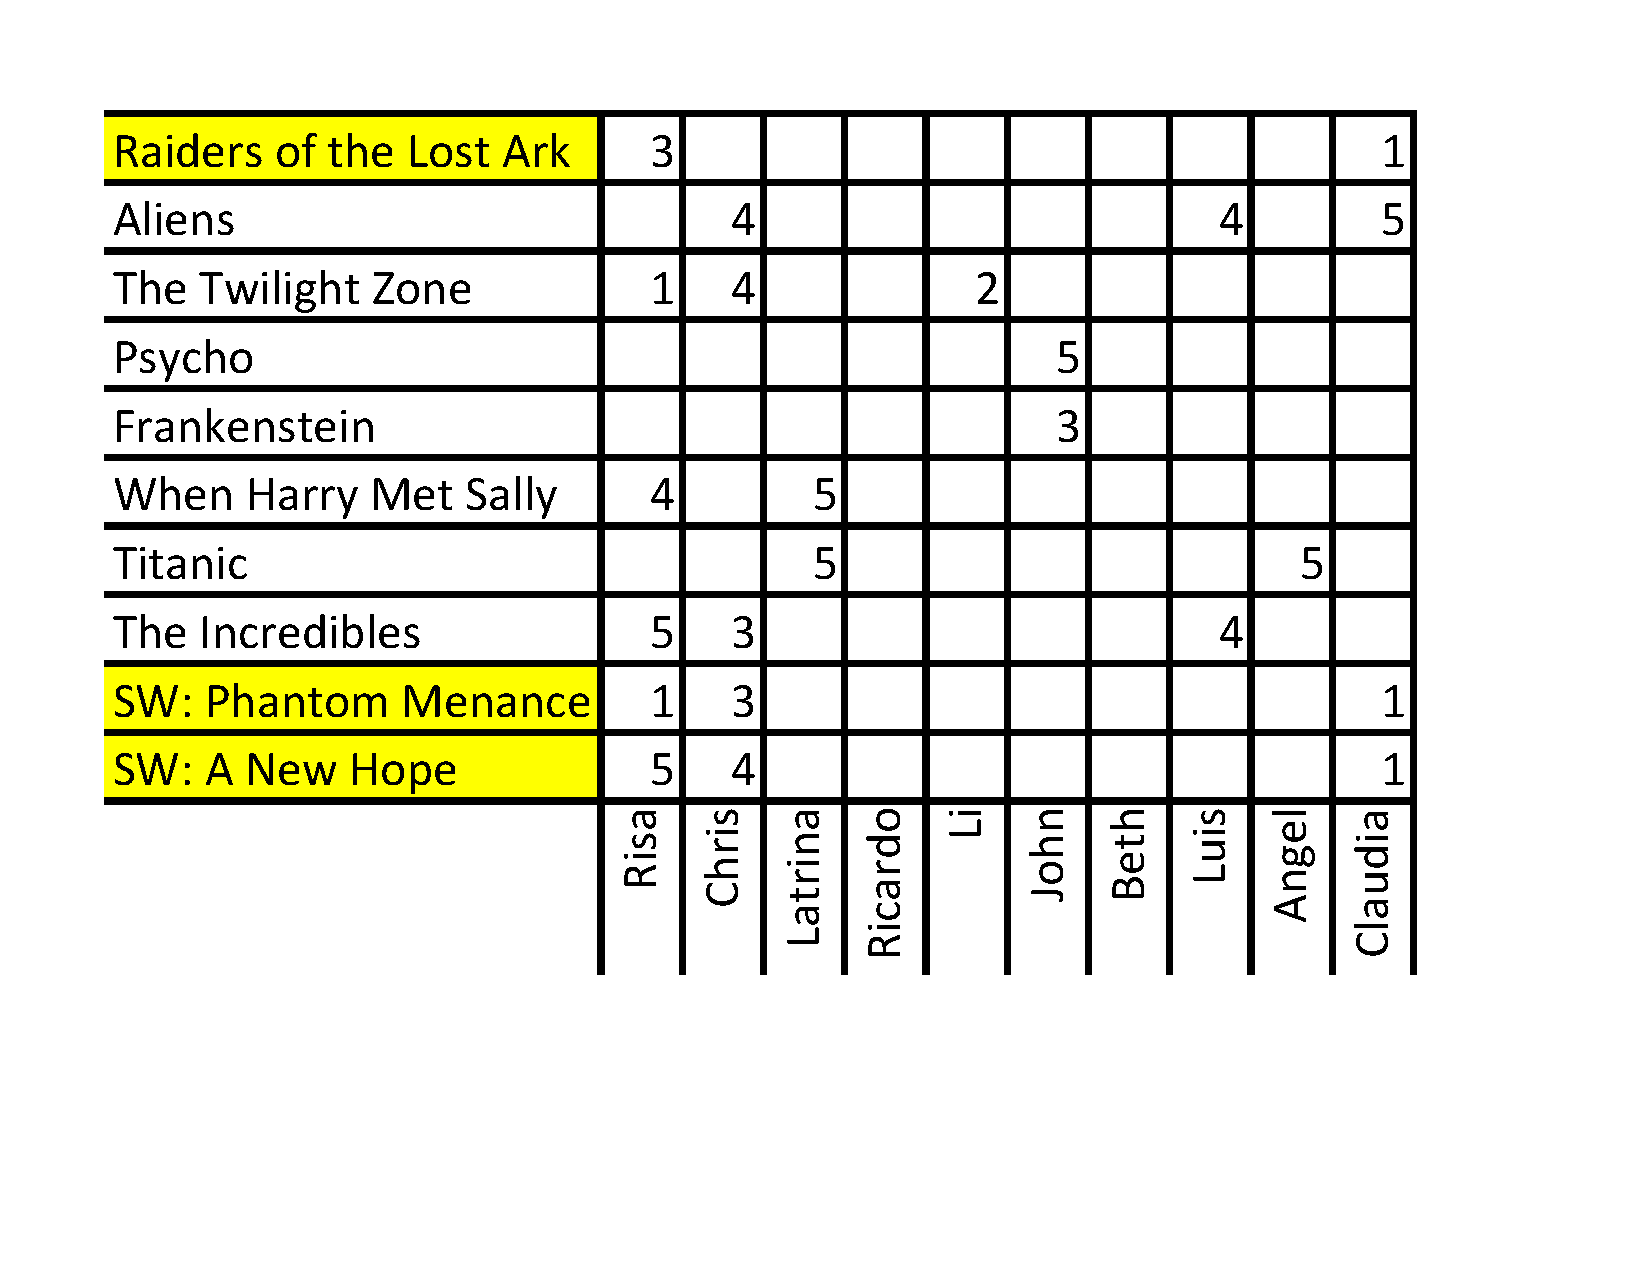
\includegraphics[width=1\textwidth]{lectUL/movieGrid2} 
\end{column}
\end{columns}

\end{frame}
%***********************************************************
\begin{frame}{Classically Two Types of Unsupervised Learning}

\begin{columns}
\begin{column}{0.5\textwidth}
\begin{enumerate}
\item Clustering
	\begin{itemize}
	\item Grouping similar points together
	\end{itemize}
\item Latent Variable methods
	\begin{itemize}
		\item Learning a model where some unseen variable helps describe the data
		\item Example: Gaussian Mixture Model - cluster identity
		\begin{itemize}
			\item Cluster identity is an unseen variable
			\item Algorithm is grouping points together
		\end{itemize}
	\end{itemize}
\end{enumerate}
\end{column}
\begin{column}{0.5\textwidth}
   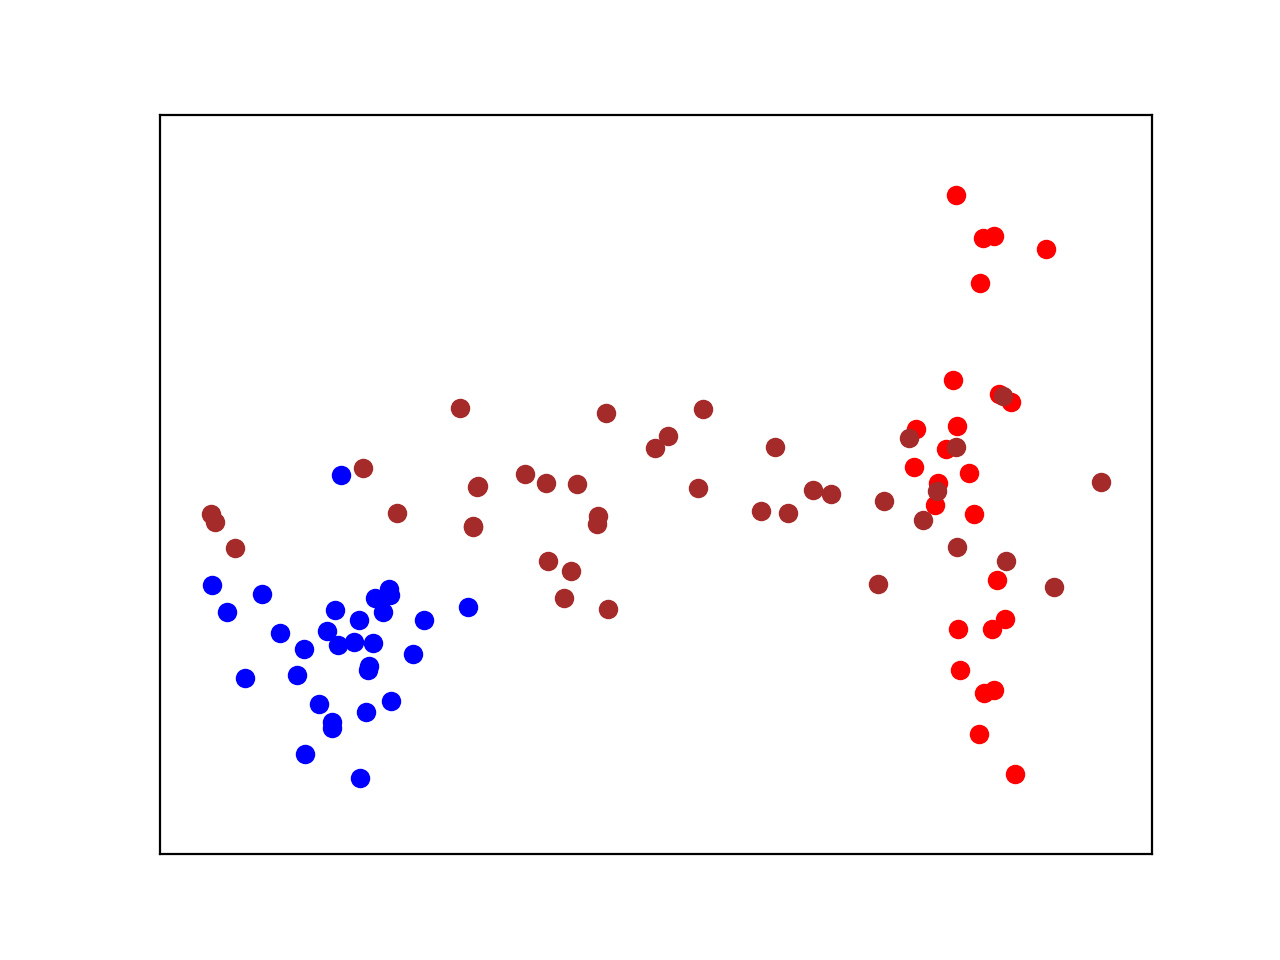
\includegraphics[width=1\textwidth]{lectUL/gaussianMixtureData.png} 
	\end{column}
\end{columns}


\end{frame}
%***********************************************************
\begin{frame}{Clustering}

\begin{itemize}
\item Goal is to group similar points together
\begin{itemize}
\item Classic method is hierarchical clustering

\item Also known as agglomerative clustering
\begin{itemize}
\item Recursively combine similar items
\item Using a distance measure
\end{itemize}\item Results in a so-called ``Dendrogram''
\item example...
\end{itemize}
\end{itemize}

\end{frame}
%***********************************************************
\begin{frame}{Hierarchical Clustering}

\begin{columns}
\begin{column}{0.5\textwidth}
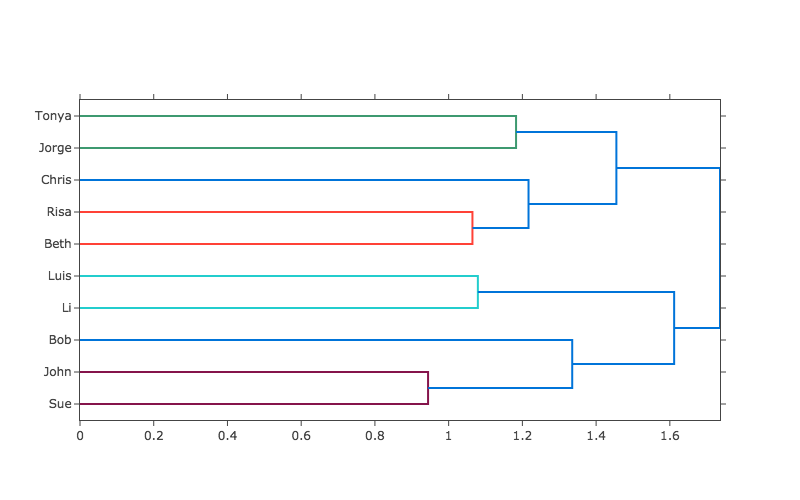
\includegraphics[width=1\textwidth]{./lectUL/dendrogram.png}
\end{column}
\begin{column}{0.5\textwidth}
\begin{itemize}
\item Define a distance measure
\item Combine the closest clusters
\item Repeat
\end{itemize}
\end{column}
\end{columns}

\end{frame}
%***********************************************************
\begin{frame}[fragile]{Hierarchical Clustering}

\begin{itemize}
\item Basic Algorithm:
\end{itemize}

\begin{SQL}
while num_clusters > 1 do
  // $D$ is the distance function
  find clusters $X$, $Y$ that minimize $D(X, Y)$
  join them
end
\end{SQL}

\begin{itemize}
\item Super-simple
\item[?] How to define cluster distance?
\end{itemize}

\end{frame}
%***********************************************************
\begin{frame}{Single-Linkage Clustering}

\begin{itemize}
\item ``Optimistic''
\begin{itemize}
	\item $D(X, Y)$ is distance between two closest points in $X$, $Y$
	\item That is, 
	$$D(X, Y) = \min_{x \in X, y \in Y} d(x, y)$$
	\item Basically Kruskal's algorithm
\end{itemize}
\end{itemize}
\end{frame}
%***********************************************************
\begin{frame}[fragile]{Single-Linkage Clustering}

\begin{itemize}
\item ``Optimistic''
\item Bottom up
\begin{itemize}
	\item $D(X, Y)$ is distance between two closest points in $X$, $Y$
	\item That is, 
	$$D(X, Y) = \min_{x \in X, y \in Y} d(x, y)$$
	\item Basically Kruskal's algorithm 
	\begin{itemize}
	\item Computes a minimum-spanning tree
	\item Finds the lowest weight edge between two nodes
	\item Greedy algorithm
	\end{itemize}
\end{itemize}
\end{itemize}

\end{frame}
%***********************************************************
\begin{frame}{Minimum Spanning Tree}

\begin{columns}
\begin{column}{0.5\textwidth}
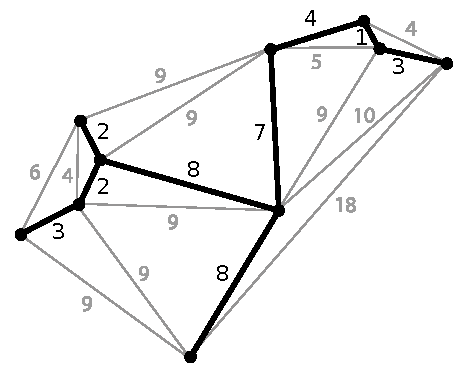
\includegraphics[width=1\textwidth]{./lectUL/Minimum_spanning_tree.pdf}
\end{column}
\begin{column}{0.5\textwidth}
\begin{itemize}
\item Subset of edges in a weighted, undirected graph 
\item Connects all the vertices
\item Using the minimum edge weights
\end{itemize}
\end{column}
\end{columns}

\end{frame}
%***********************************************************
\begin{frame}{Greedy Algorithm}

\begin{columns}
\begin{column}{0.5\textwidth}
\begin{itemize}
\item Goal: Find the highest value path to the bottom of the tree
\item Greedy Approach: Pick the best available option
\end{itemize}
\end{column}
\begin{column}{0.5\textwidth}
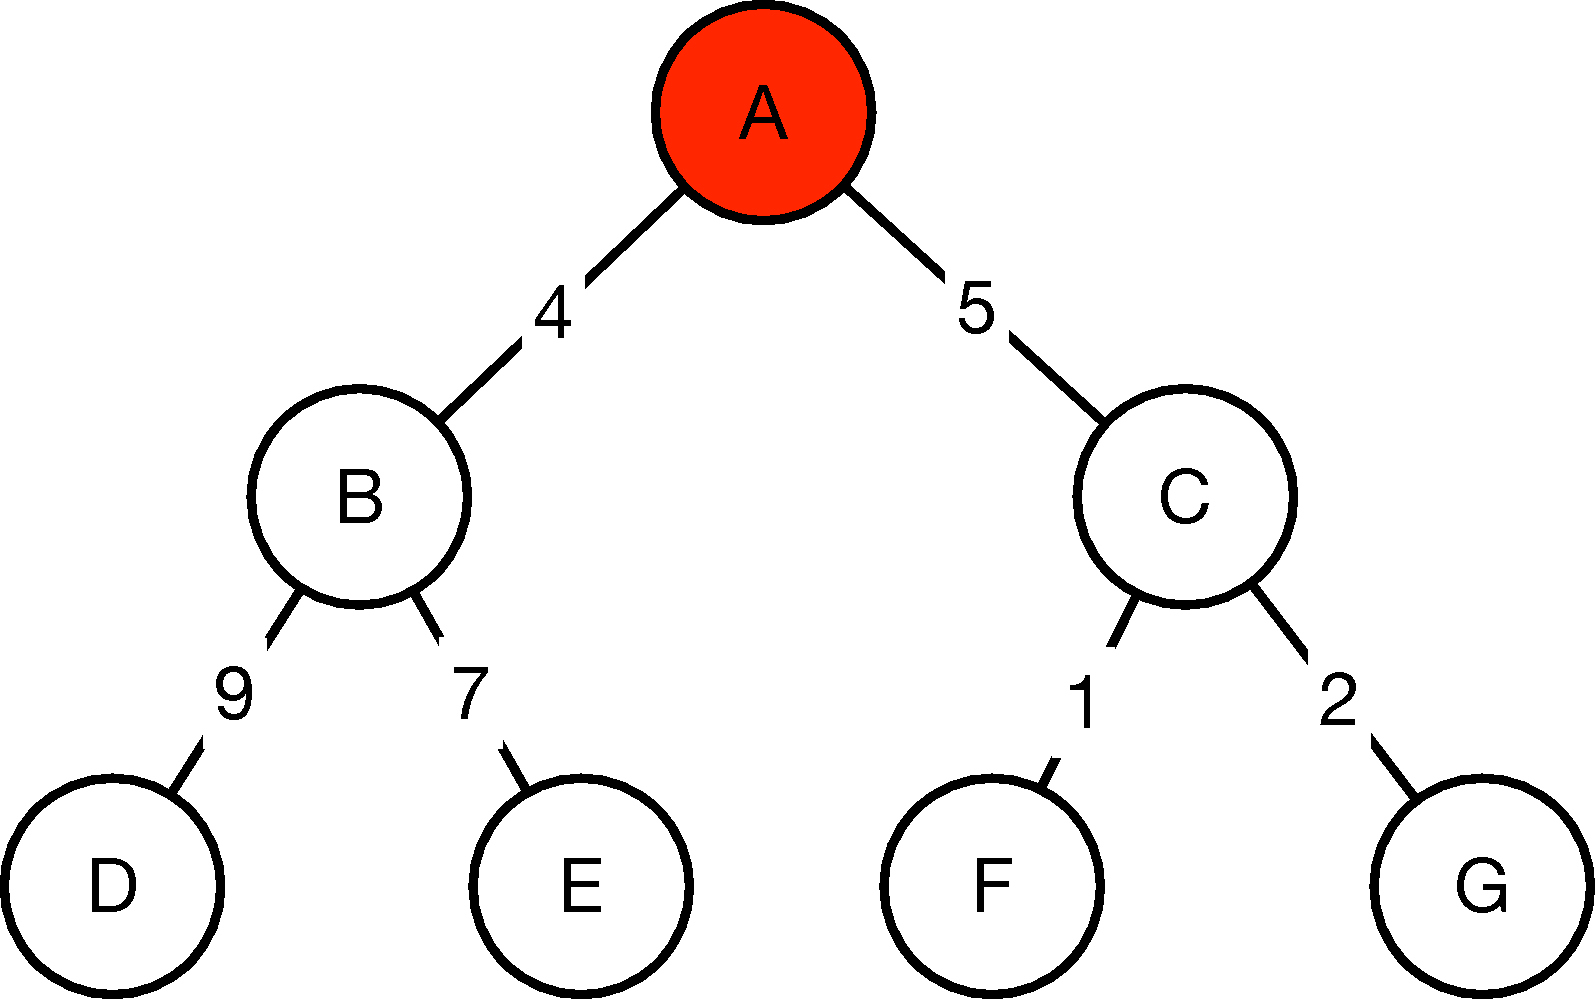
\includegraphics[width=1\textwidth]{./lectUL/greedy1.pdf}
\end{column}
\end{columns}

\end{frame}

%***********************************************************
\begin{frame}{Greedy Algorithm}

\begin{columns}
\begin{column}{0.5\textwidth}
\begin{itemize}
\item Goal: Find the highest value path to the bottom of the tree
\item Greedy Approach: Pick the best available option
\end{itemize}
\end{column}
\begin{column}{0.5\textwidth}
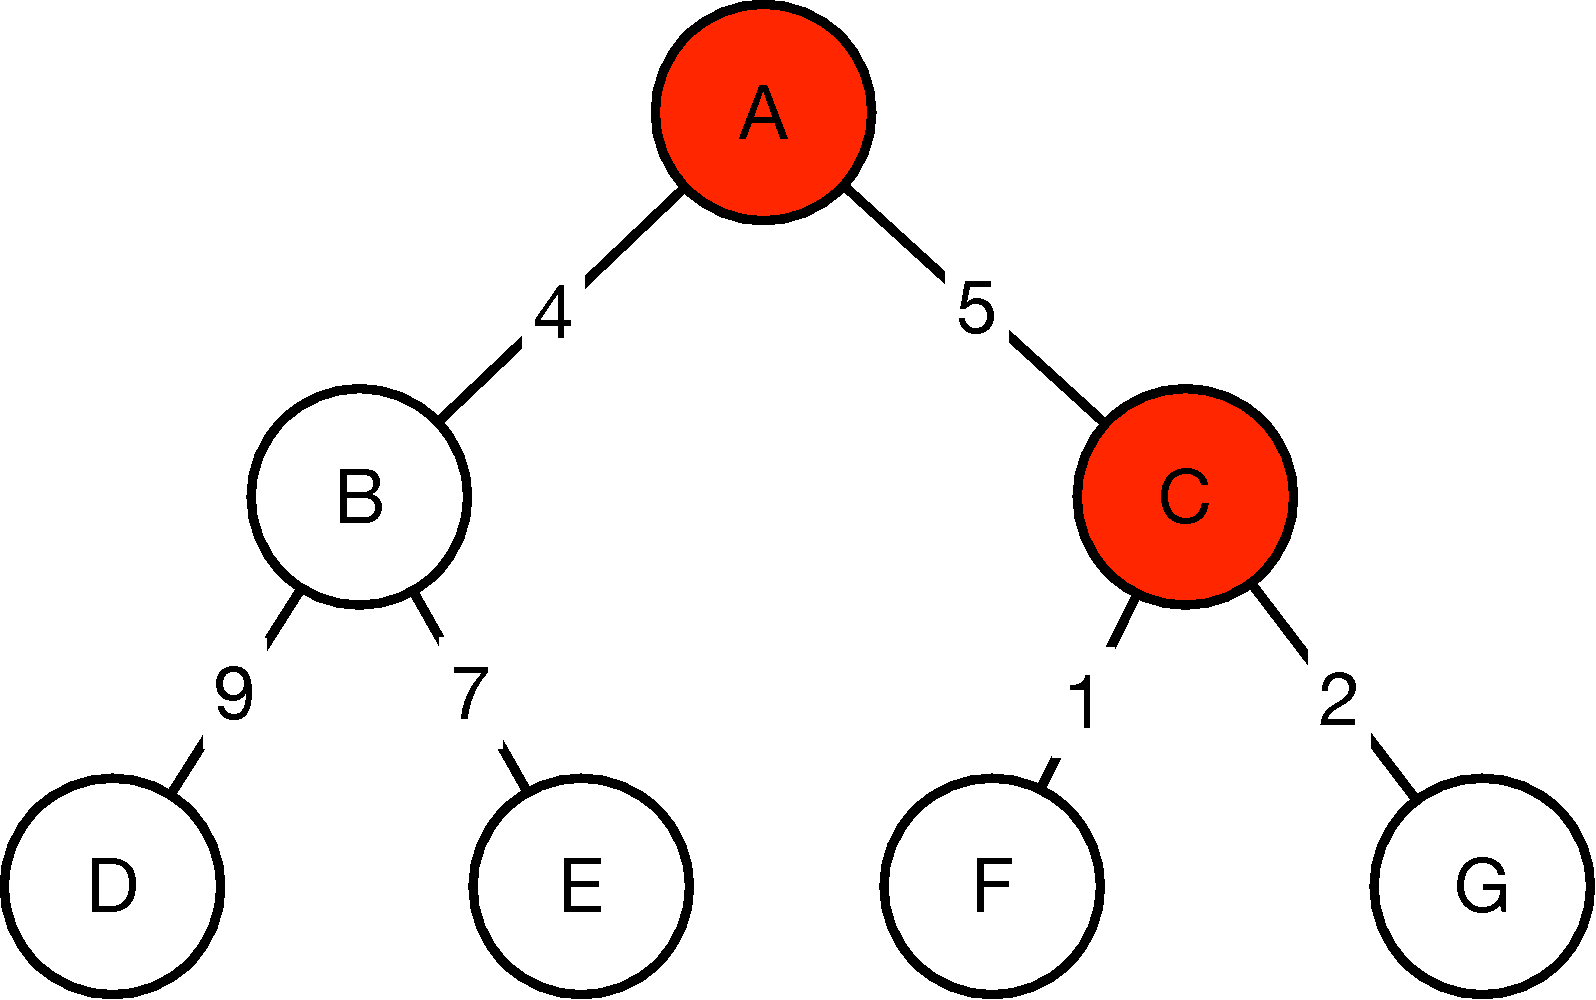
\includegraphics[width=1\textwidth]{./lectUL/greedy2.pdf}
\end{column}
\end{columns}

\end{frame}
%***********************************************************
\begin{frame}{Greedy Algorithm}

\begin{columns}
\begin{column}{0.5\textwidth}
\begin{itemize}
\item Goal: Find the highest value path to the bottom of the tree
\item Greedy Approach: Pick the best available option
\end{itemize}
\end{column}
\begin{column}{0.5\textwidth}
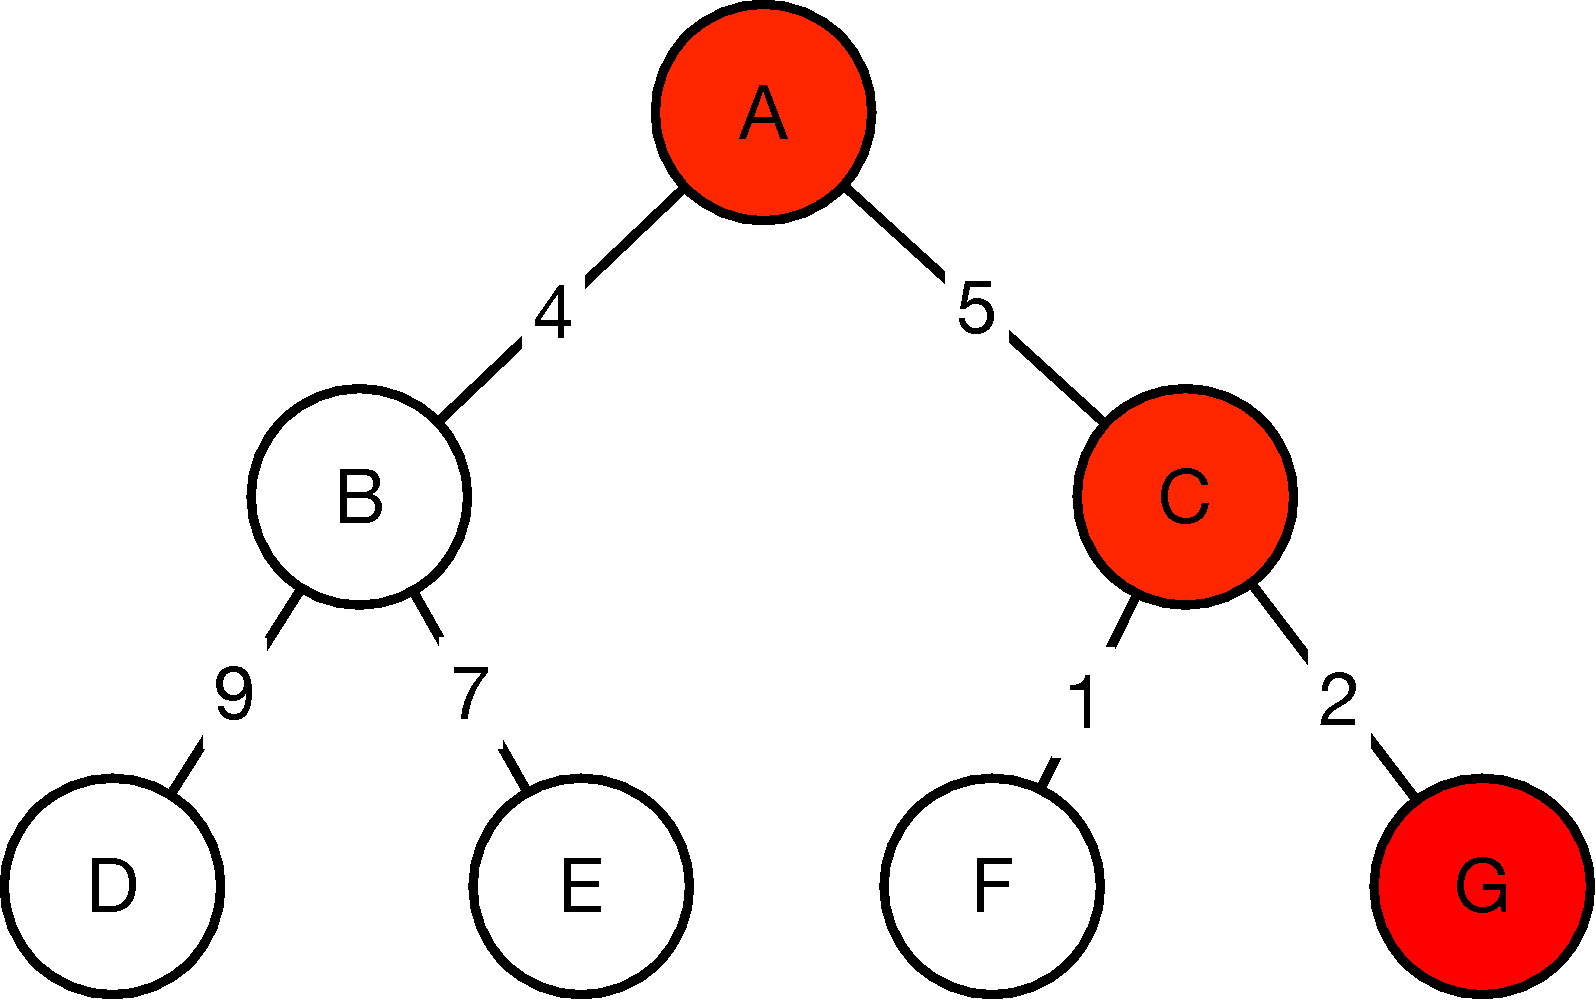
\includegraphics[width=1\textwidth]{./lectUL/greedy3.pdf}
\end{column}
\end{columns}

\end{frame}
%***********************************************************
\begin{frame}{Greedy Algorithm}

\begin{columns}
\begin{column}{0.5\textwidth}
\begin{itemize}
\item[?] Advantages?
\end{itemize}
\end{column}
\begin{column}{0.5\textwidth}
\begin{itemize}
\item[?] Disadvantages?
\end{itemize}
\end{column}
\end{columns}

\end{frame}
%***********************************************************
\begin{frame}{Greedy Algorithm}

\begin{columns}
\begin{column}{0.5\textwidth}
\begin{itemize}
\item Advantages?
\begin{itemize}
\item Simple
\item Fast
\end{itemize}
\end{itemize}
\end{column}
\begin{column}{0.5\textwidth}
\begin{itemize}
\item Disadvantages?
\begin{itemize}
\item Often don't find the best solution
\item Non-recoverable % once you are heading down the wrong path, you typically can't fix it
\end{itemize}
\end{itemize}
\end{column}
\end{columns}

\end{frame}



%***********************************************************
\begin{frame}{Single-Linkage Clustering}

\begin{columns}
\begin{column}{0.5\textwidth}
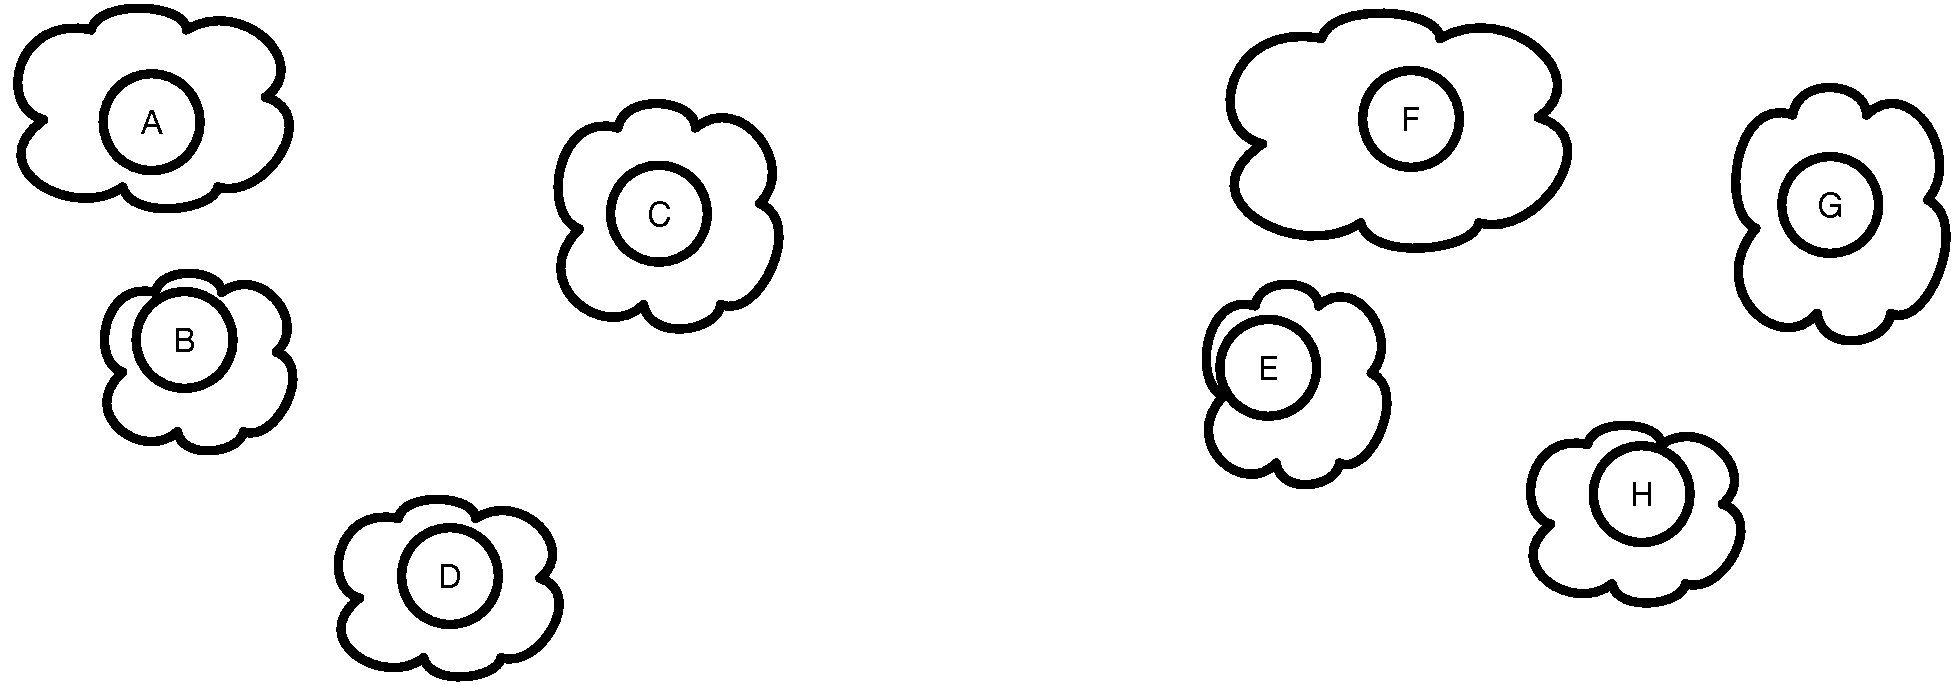
\includegraphics[width=1\textwidth]{./lectUL/minLinkageClustering1.pdf}
\end{column}
\begin{column}{0.5\textwidth}
\begin{itemize}
\item Each point is in its own cluster
\end{itemize}
\end{column}
\end{columns}
\end{frame}
%***********************************************************
\begin{frame}{Single-Linkage Clustering}

\begin{columns}
\begin{column}{0.5\textwidth}
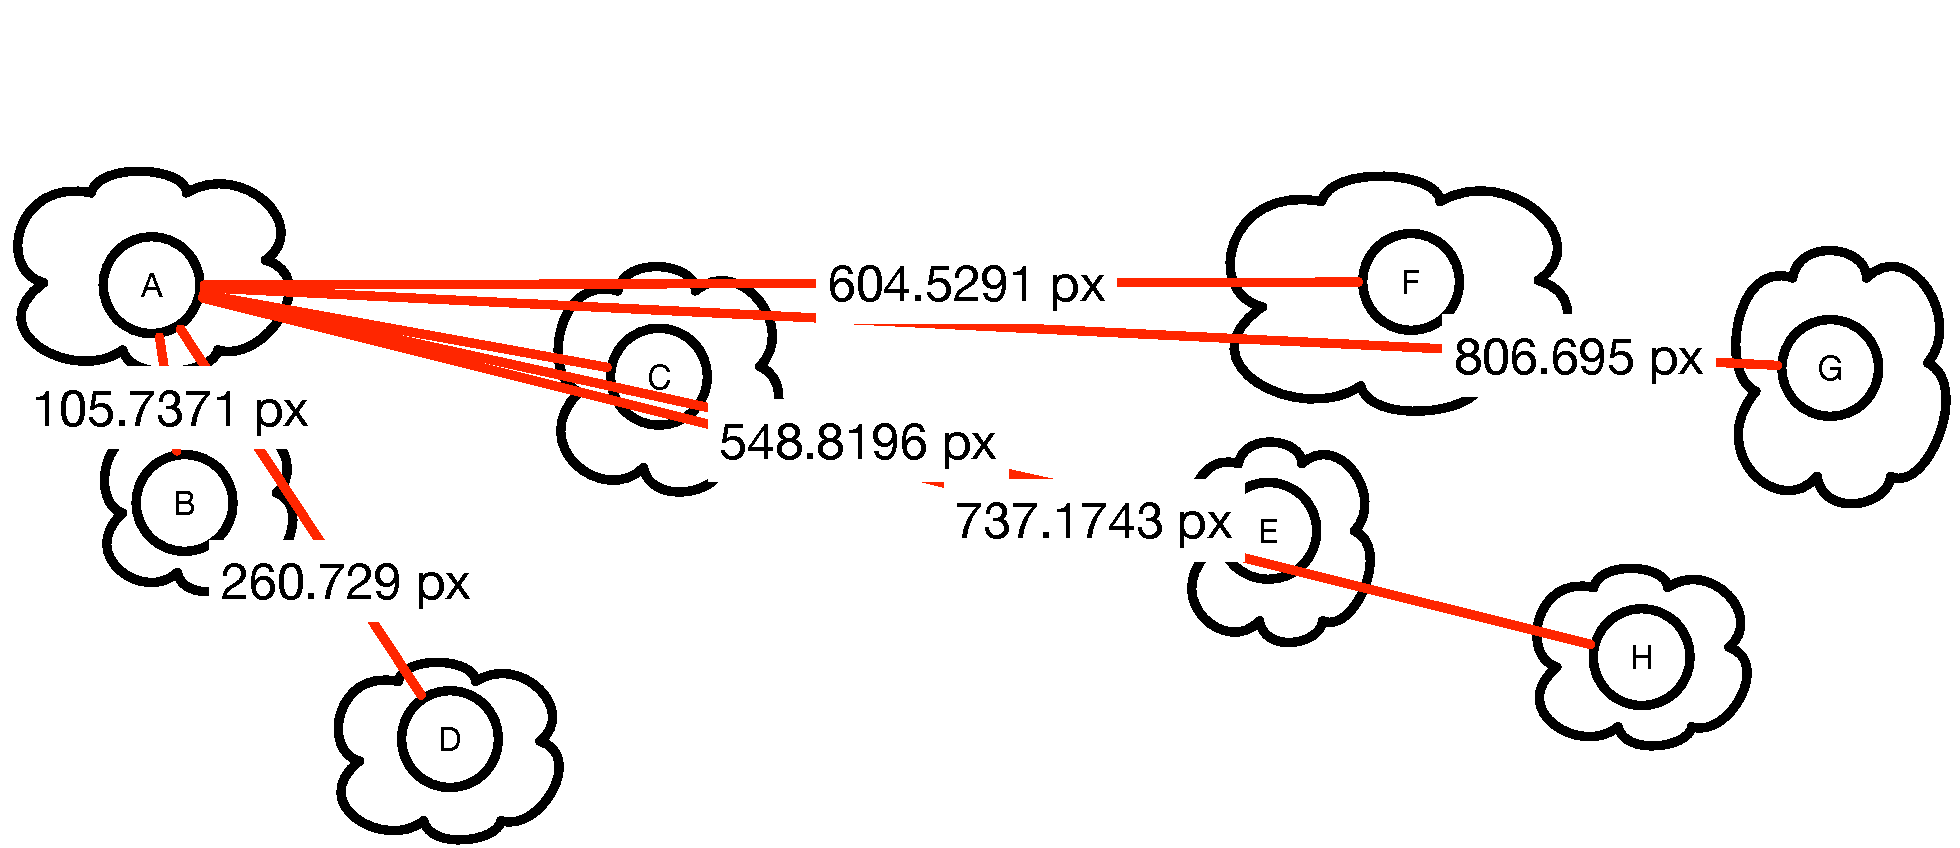
\includegraphics[width=1\textwidth]{./lectUL/minLinkageClustering2.pdf}
\end{column}
\begin{column}{0.5\textwidth}
\begin{itemize}
\item Compute the distance between EVERY pair of points
\begin{tabular}{|r|r|r|} \hline
Point & Point & Distance \\ \hline
A & B & 105\\ \hline
A & C & 260 \\ \hline
B & C & 236 \\ \hline
$\ldots$ & $\ldots$  & $\ldots$ \\ \hline
\end{tabular}
\end{itemize}
\end{column}
\end{columns}
\end{frame}
%***********************************************************
\begin{frame}{Single-Linkage Clustering}

\begin{columns}
\begin{column}{0.5\textwidth}
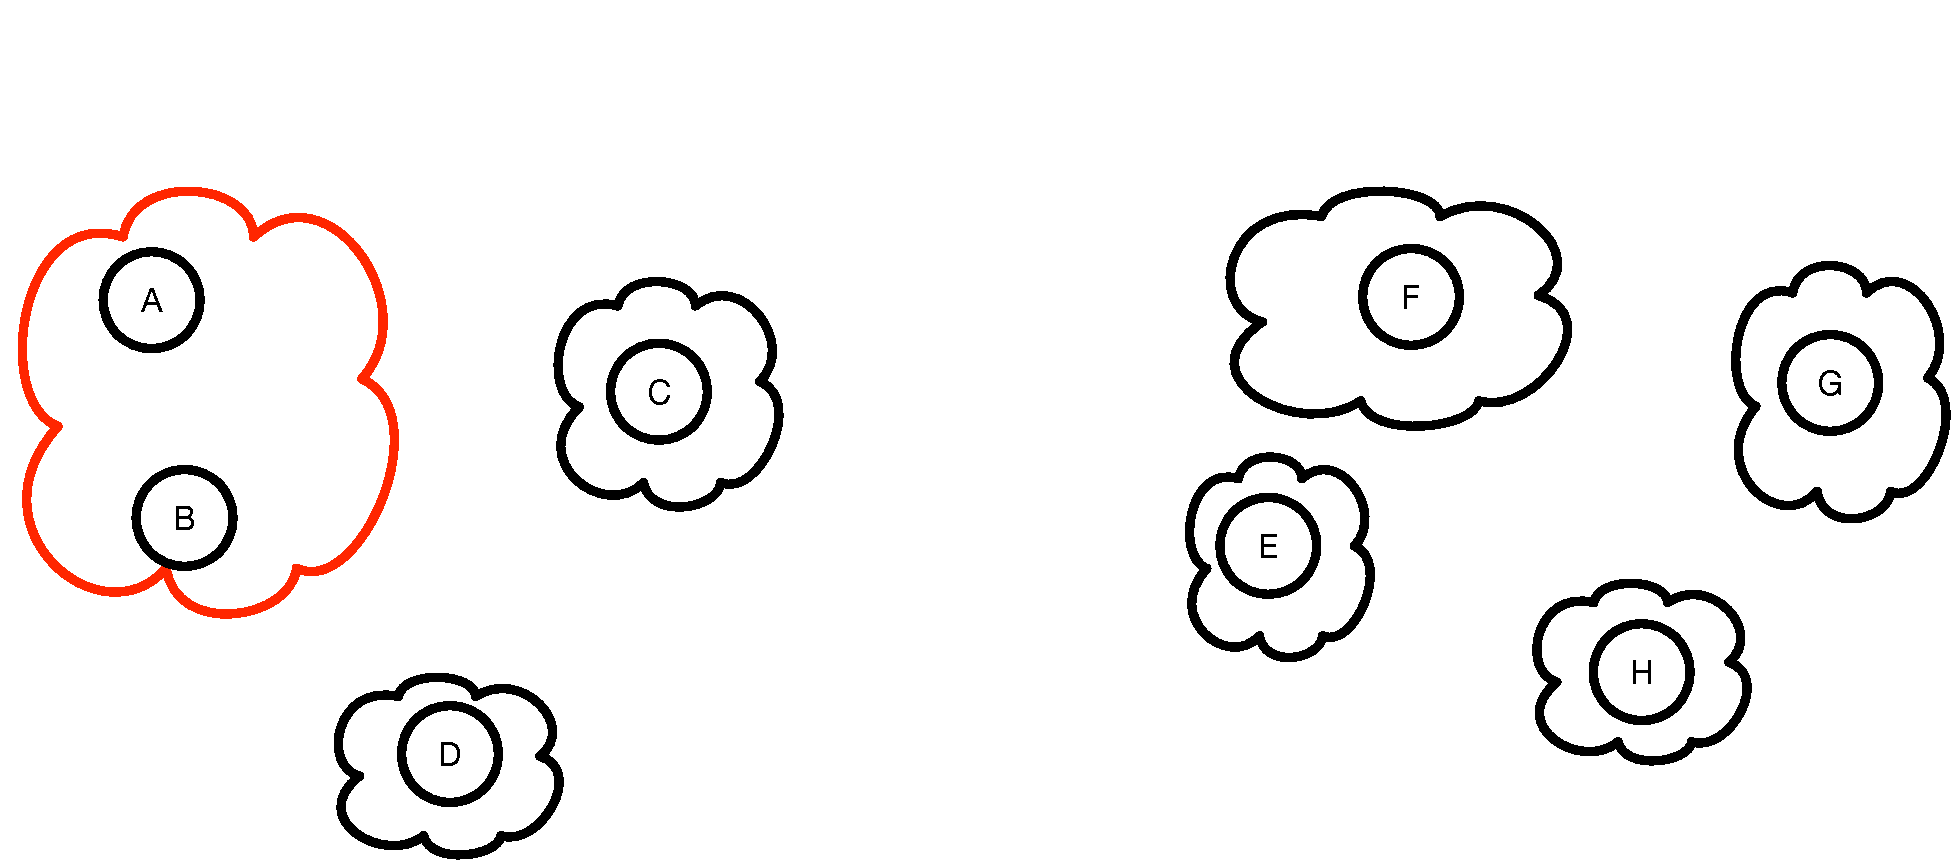
\includegraphics[width=1\textwidth]{./lectUL/minLinkageClustering3.pdf}
\end{column}
\begin{column}{0.5\textwidth}
\begin{itemize}
\item Cluster together the two closest points
\item Use the distance from the closest point in each cluster to the closest point in the other clusters
\item Repeat until the number of clusters = 1
\end{itemize}
\end{column}
\end{columns}
\end{frame}
%***********************************************************
\begin{frame}{Single-Linkage Clustering}

\begin{itemize}
\item ``Optimistic''
\begin{itemize}
	\item $D(X, Y)$ is distance between two closest points in $X$, $Y$
	\item That is, 
	$$D(X, Y) = \min_{x \in X, y \in Y} d(x, y)$$
	\item Basically Kruskal's algorithm
\end{itemize}
\item Drawbacks?
	\begin{itemize}
	\item Naive solution $O(n^3)$ % can't use for big data
	\item ...Possible to use variant of Prim's algorithm to get $O(n^2)$
	\item ``Chaining''
	\end{itemize}
\end{itemize}
\end{frame}
%***********************************************************
\begin{frame}{Single-Linkage Example}

\begin{columns}
\begin{column}{0.5\textwidth}
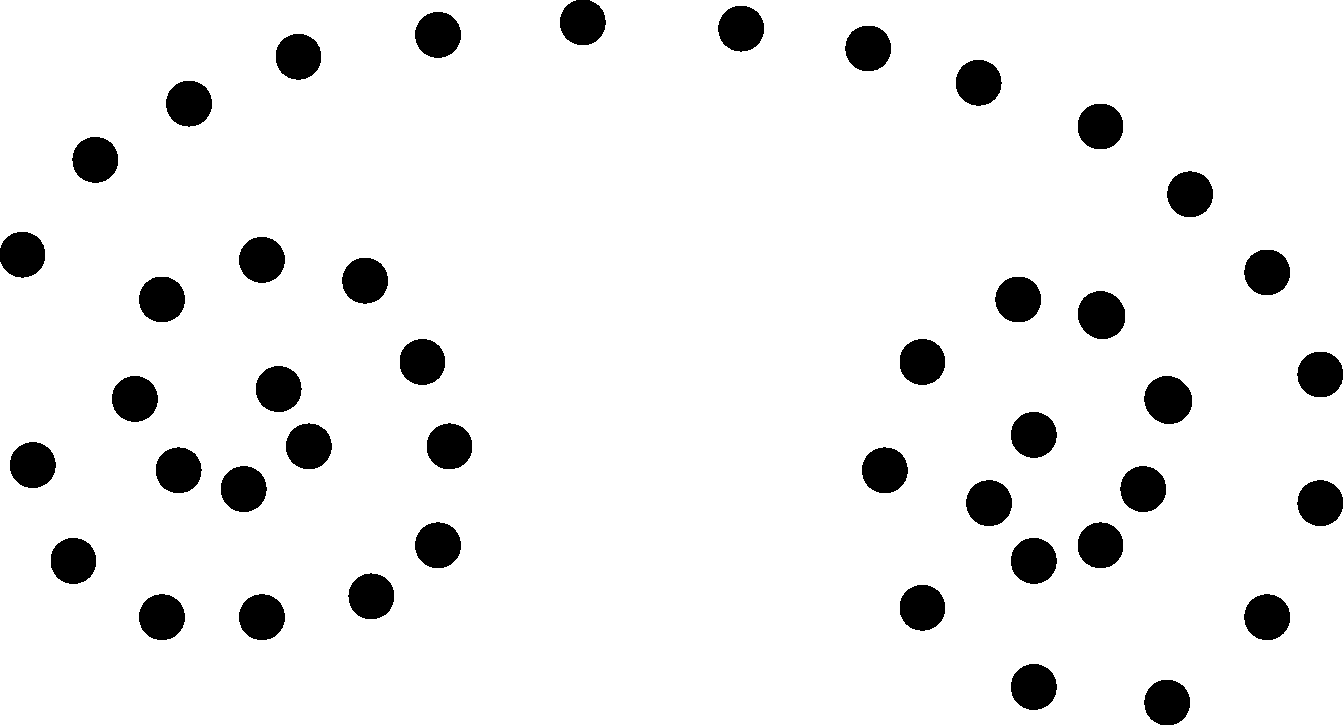
\includegraphics[width=1\textwidth]{./lectUL/singleLinkNoGroups.pdf}
\end{column}
\begin{column}{0.5\textwidth}
\begin{itemize}
\item How would you cluster this data, if you grouped the closest points  / groups each time?
\item Show the penultimate 2  groups
\end{itemize}
\end{column}
\end{columns}
\end{frame}
%***********************************************************
\begin{frame}{Single-Linkage Drawback: Chaining}

\begin{columns}
\begin{column}{0.5\textwidth}
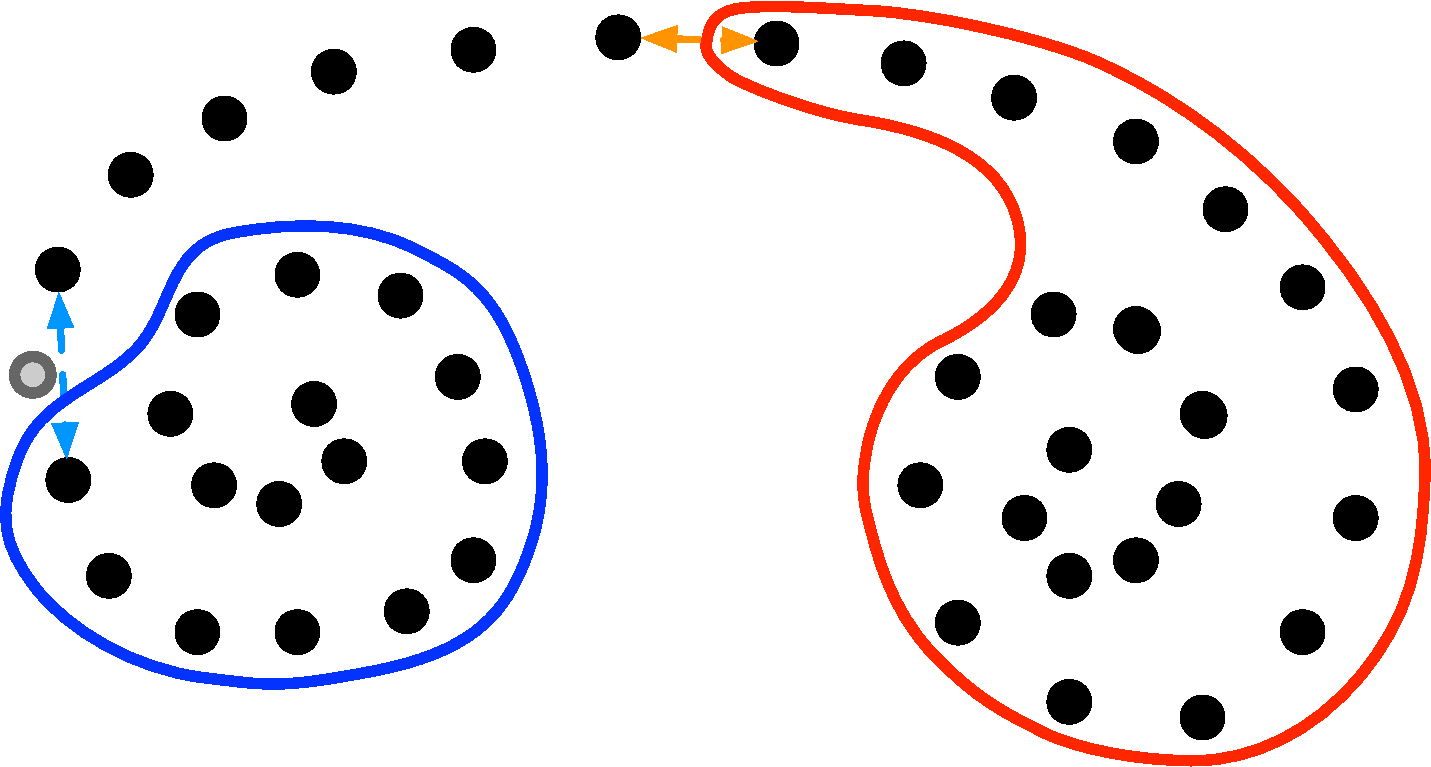
\includegraphics[width=1\textwidth]{./lectUL/singleLink1.pdf}
\end{column}
\begin{column}{0.5\textwidth}
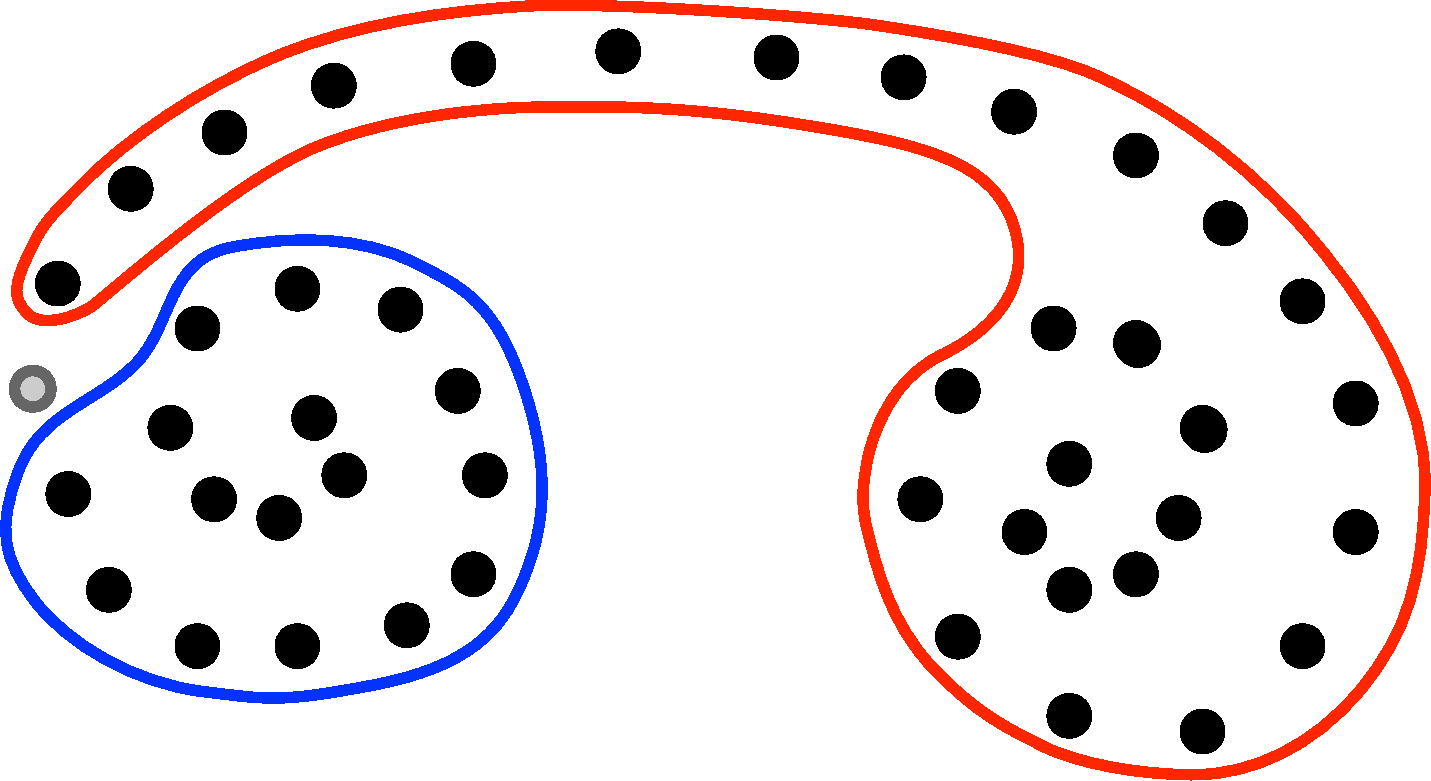
\includegraphics[width=1\textwidth]{./lectUL/singleLink2.pdf}
\end{column}
\end{columns}
\end{frame}
%***********************************************************
\begin{frame}{Single-Linkage Drawback: Chaining}

\begin{columns}
\begin{column}{0.5\textwidth}
Actual\\
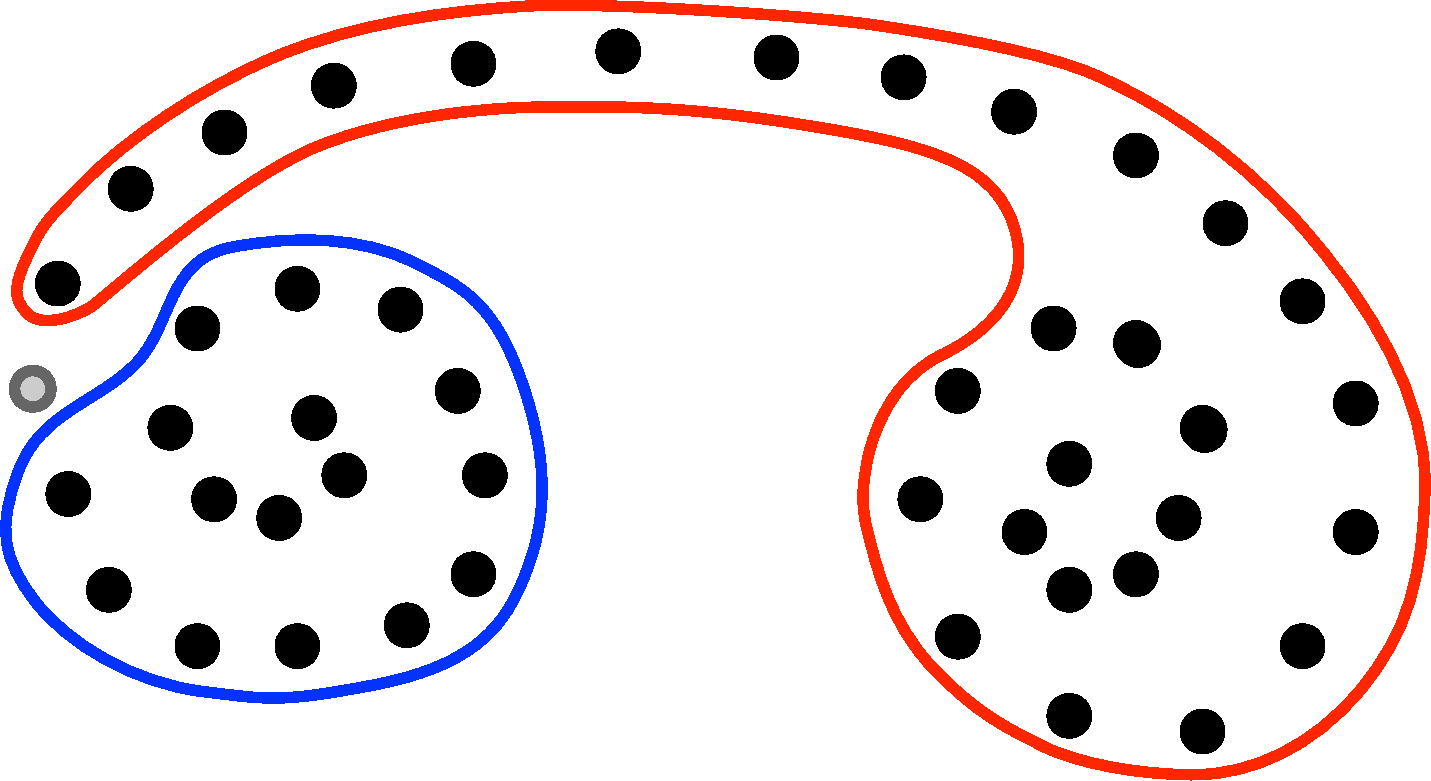
\includegraphics[width=1\textwidth]{./lectUL/singleLink2.pdf}
\end{column}
\begin{column}{0.5\textwidth}
Expected\\
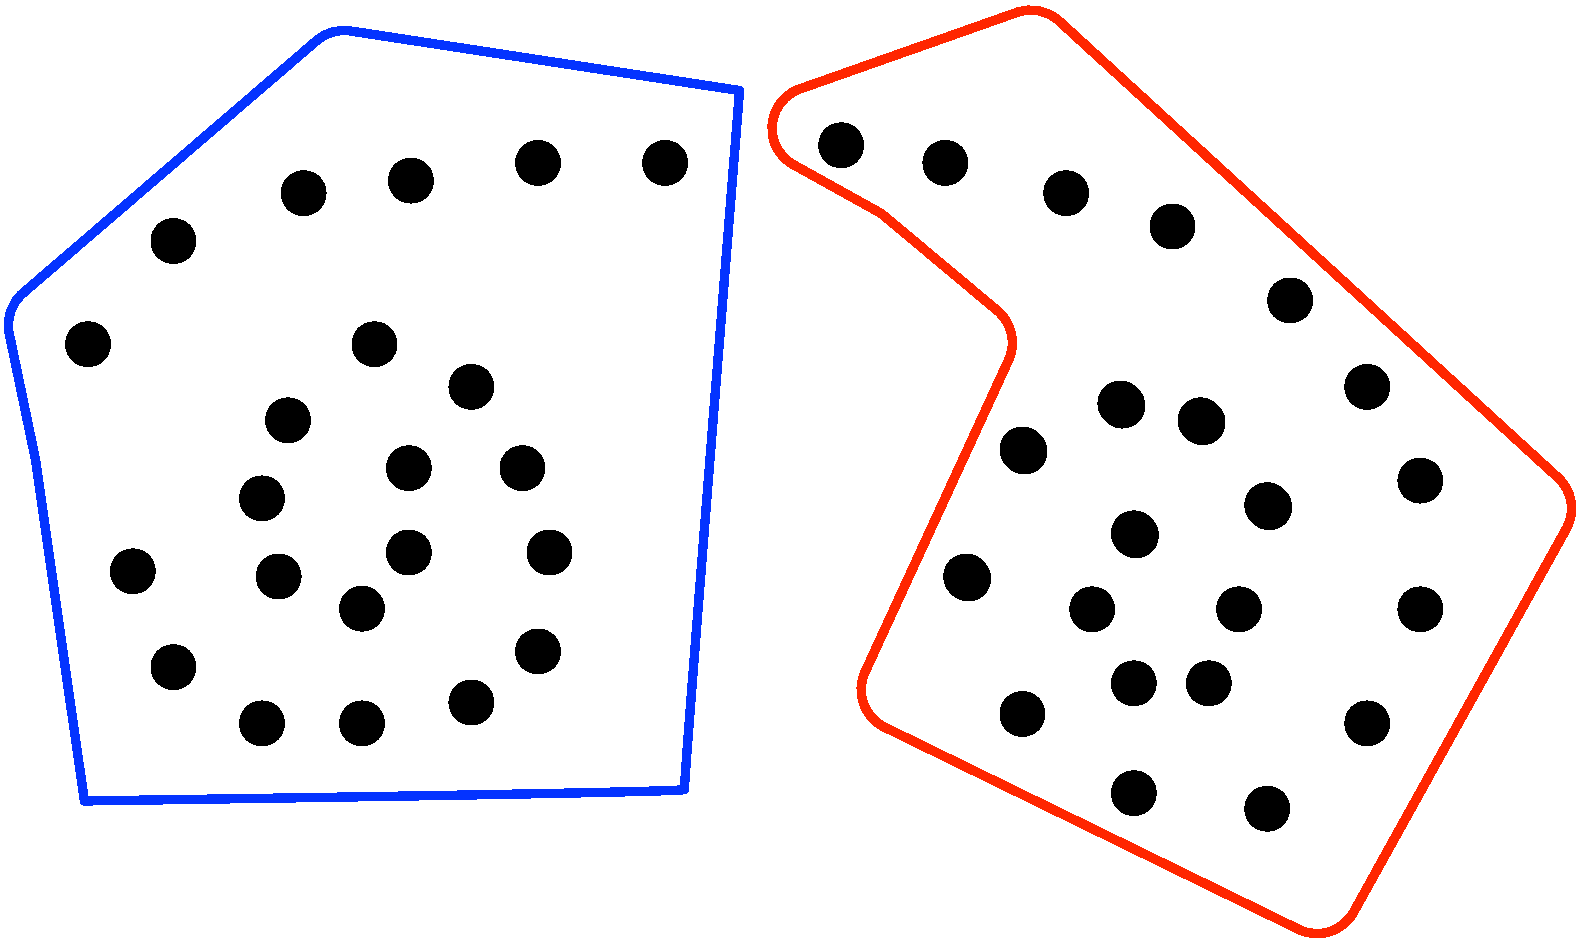
\includegraphics[width=1\textwidth]{./lectUL/singleLinkExpected.pdf}
\end{column}
\end{columns}
\end{frame}
%***********************************************************
\begin{frame}{Complete-Linkage Clustering}

\begin{itemize}
\item ``Pessimistic''
\item Also known as farthest neighbor clustering
\item Start with each point in its own cluster
\begin{itemize}
	\item $D(X, Y)$ is distance between two \textcolor {red}{most distant} points in $X$, $Y$
	\item That is, 
	$$D(X, Y) = \max_{x \in X, y \in Y} d(x, y)$$
	\item Tends to produce more compact clusterings
	\item Best solution is also $O(n^2)$
\end{itemize}
\end{itemize}

\end{frame}
%***********************************************************
\begin{frame}{Single vs. Complete-Linkage Clustering}

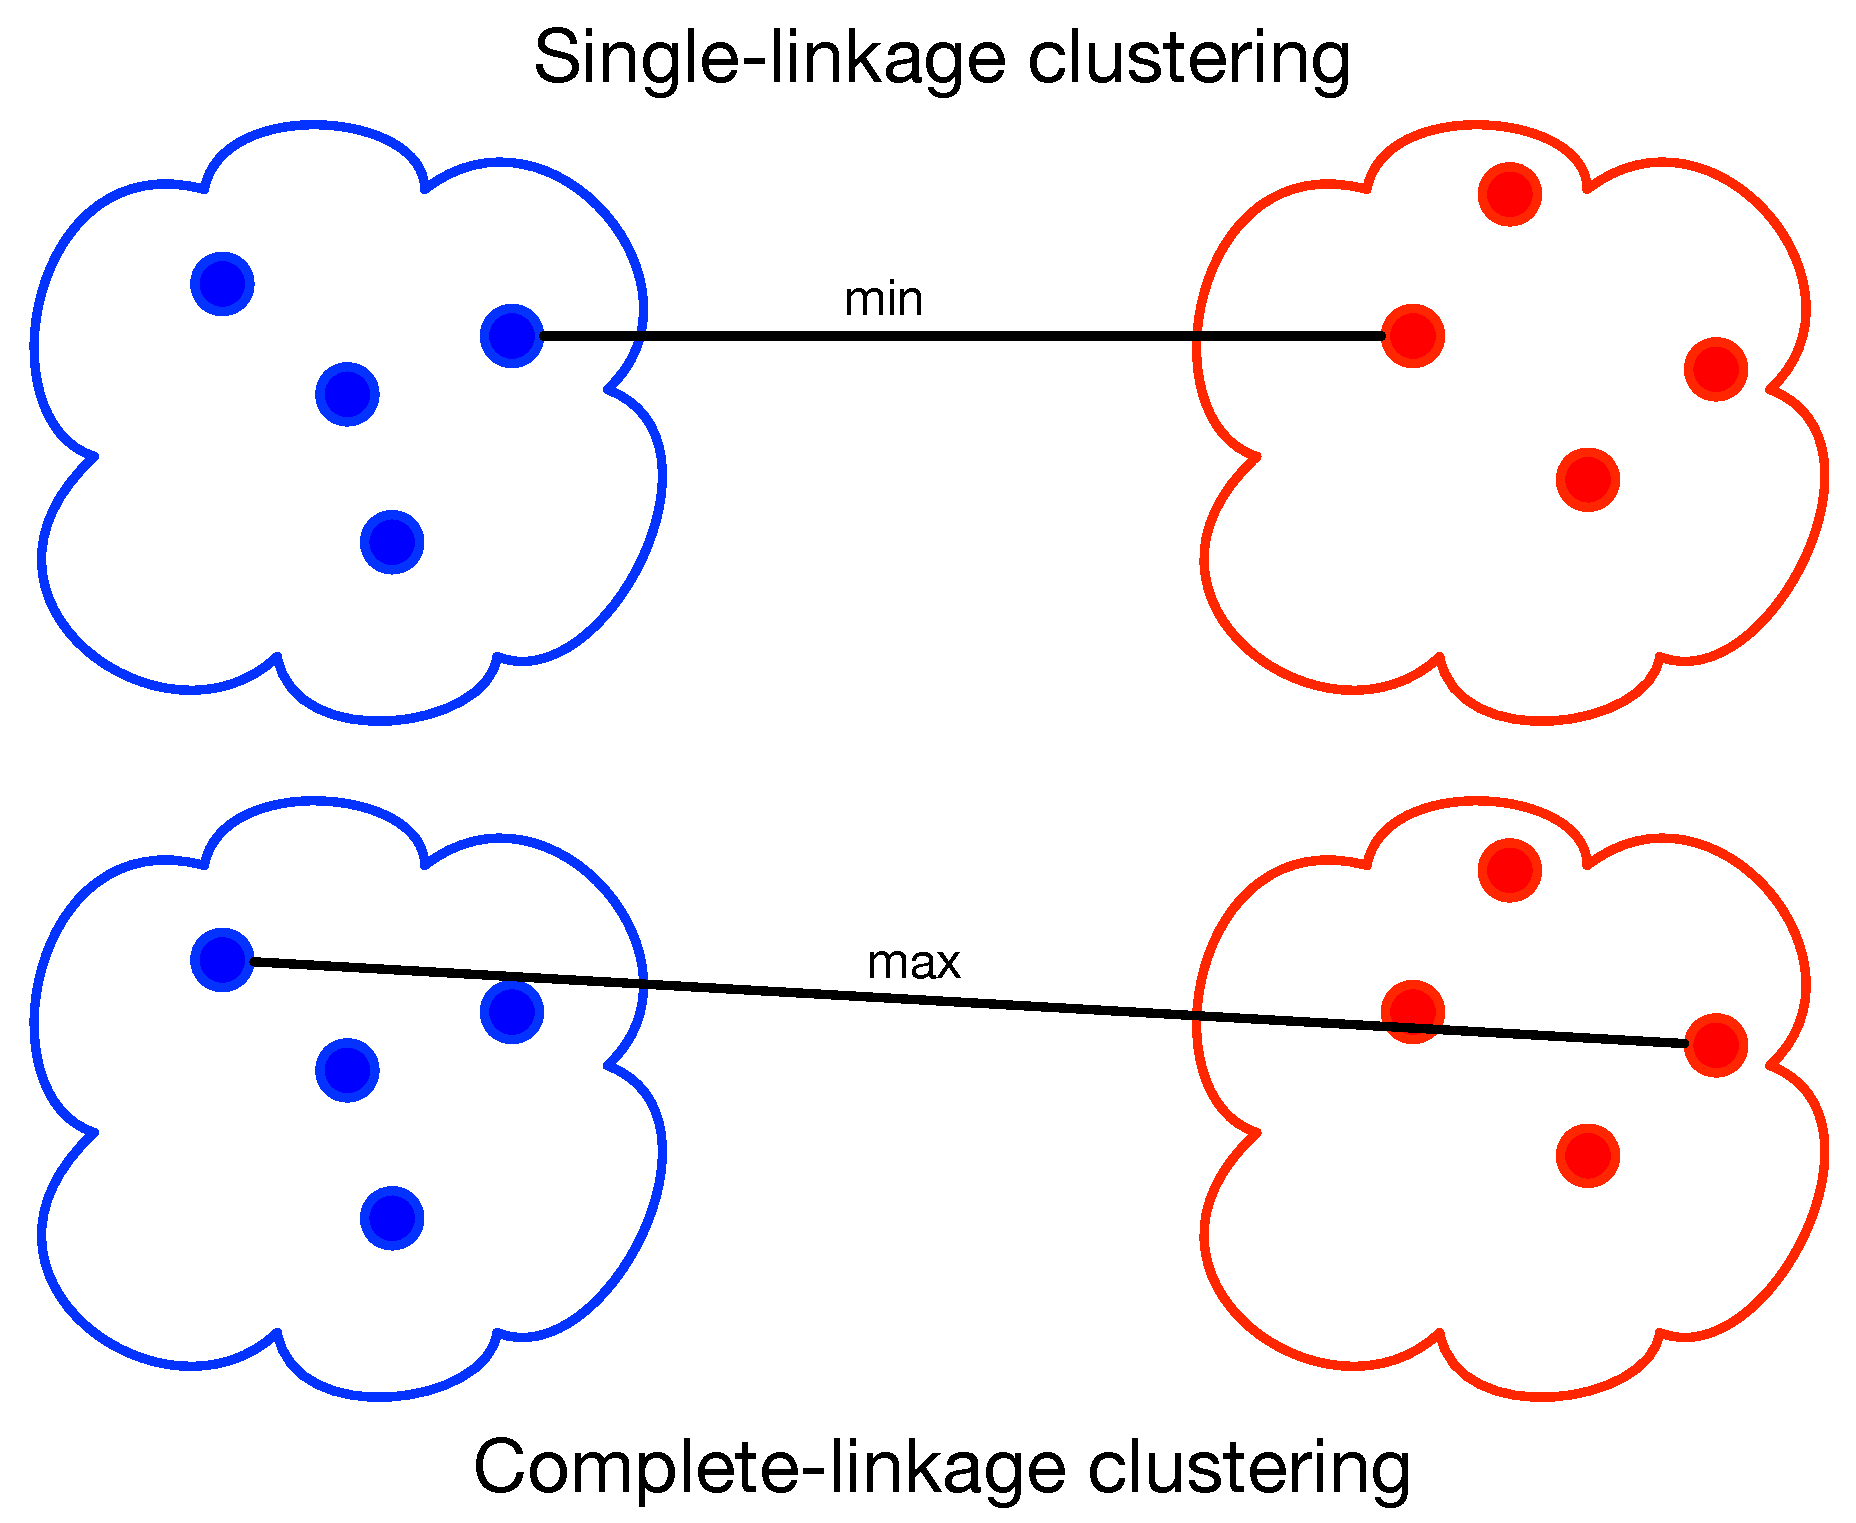
\includegraphics[width=.65\textwidth]{./lectUL/compareLinkageClustering.pdf}
\end{frame}

%***********************************************************
\begin{frame}{What About The Distance?}

\begin{itemize}
\item How to compute $d(x, y)$?
	\begin{itemize}
	\item Classical method: if $x$, $y$ vectors, use $l_p$ norm of $x - y$
	\item[?] Drawbacks?
	\end{itemize}
\end{itemize}



\end{frame}
%***********************************************************
\begin{frame}{What About The Distance?}

\begin{itemize}
\item How to compute $d(x, y)$?
	\begin{itemize}
	\item Classical method: if $x$, $y$ vectors, use $l_p$ norm of $x - y$
	\item Drawbacks?
	\begin{itemize}
	\item All factors have the same weight
	\item Consider shoe size: child: 4 - 13 basketball player
	\item Versus weight: child: 40 lbs - 250 lbs basketball player
	\end{itemize}
	\end{itemize}
\end{itemize}
\end{frame}

%***********************************************************
\begin{frame}{Normalize the factors}

\begin{itemize}
\item Frequently addressed by performing a Z-transform on the data
\item Subtract out the mean
\item Divide every factor, $x_i$ by the standard deviation of the data
$$ z_i = \frac{x_i - \bar{x}}{s}$$

\end{itemize}
\end{frame}
%%***********************************************************
%\begin{frame}{More Drawbacks to the Distance?}
%
%\begin{itemize}
%\item Attributes tend to cluster into bunches that are not all that different from each other
%\end{itemize}
%\end{frame}

%***********************************************************
\begin{frame}{What About The Distance?}

\begin{itemize}
\item Mahalanobis distance is more robust
	\begin{itemize}
	\item Let $\mu$ be the mean vector of the data set
	\item Let $S$ be the observed covariance matrix of data set
	\item That is, let $X$ be the matrix where the $i$th row is $x_i - \mu$
	\item Then $S = \frac{1}{n - 1} X^T X$ 	
	\item Mahalanobis computed as:
		$$ d(x, y) = \left((x - y)^T S^{-1} (x - y)\right)^{\frac{1}{2}}$$
	\item Intuition?
	\end{itemize}
\end{itemize}
\end{frame}
%***********************************************************
%\begin{frame}{Mahalanobis Distance Intuition}
%
%\begin{itemize}
%\item Generalization of measuring how many standard deviations away a point is
%\item Pairwise linearly transform of feature values
%\item Allows for better comparisons between dimensions
%\item Measures how far features are from each other by taking into account the covariances between the distributions of the feature values
%\item That is, the spread of the points in the set
%\item The mapping de-correlates the data by finding the axis along which the data varies the most
%\item Often used instead of Euclidean distance, especially when the scale of the features varies greatly
%\end{itemize}
%\footnote{Weinberger KQ, Saul LK. Distance Metric Learning for Large Margin Nearest Neighbor Classification. The Journal of Machine Learning Research. 2009;10:207--44.}
%\end{frame}

%***********************************************************
\begin{frame}{Mahalanobis Distance Intuition}

\begin{itemize}
\item Scenario
\begin{itemize}
\item Have a number of points in a set
\item Want to know if a new point belongs or not
\item Take into consideration the spread of the points in the set
\item If the new point is close to the center, it more likely belongs
\item If the set is not spherical in nature, we need to look at the covariance matrix
\item The Mahalanobis distance measure the distance from the new point to the weighted center of mass of the set
\end{itemize}
\end{itemize}
\end{frame}

%***********************************************************
\begin{frame}{Mahalanobis Distance Illustrated}

\begin{columns}
\begin{column}{0.5\textwidth}
Actual\\
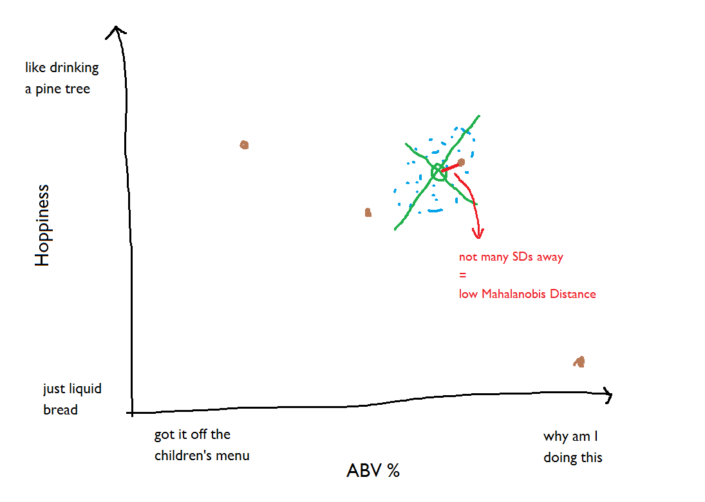
\includegraphics[width=1\textwidth]{./lectUL/mah1.png}
\end{column}
\begin{column}{0.5\textwidth}
Expected\\
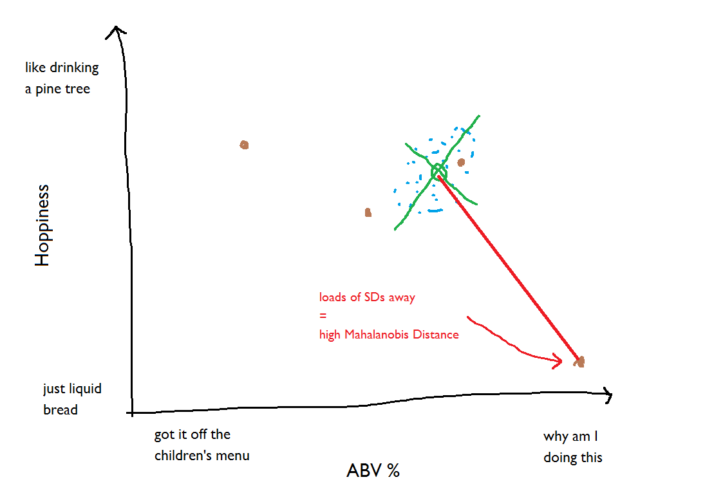
\includegraphics[width=1\textwidth]{./lectUL/mah2.png}
\end{column}
\end{columns}
https://www.theinformationlab.co.uk/2017/05/26/mahalanobis-distance/
\end{frame}


%%***********************************************************
%\begin{frame}{Other Clustering Methods?}
%
%\begin{itemize}
%\item Naturally they exist...
%\item Will talk about a few over the next few weeks!
%\end{itemize}
%
%\end{frame}
%***********************************************************
\begin{frame}{Mahalanobis Distance Intuition}
\begin{itemize}
\item Alternative to clustering
\item Latent Variable Methods
\end{itemize}
\end{frame}
%***********************************************************
\begin{frame}{Latent Variable Methods (instead of Clustering)}

\begin{itemize}
\item What is a Latent Variable Method?
	\begin{itemize}
	\item By postulating the existence of ``latent'' variables
	\item Latent: missing or unobserved %(back to the coin flip!)
	\item Difference: latent variables typically imagined
	\item Used to help simplify/explain the data
	\item Often probabilistic (MLE, Bayesian)
	\item Can be optimization-based
	\end{itemize}
\end{itemize}

\end{frame}
%***********************************************************
\begin{frame}{Classic Example: NNMF}

\begin{columns}
\begin{column}{0.5\textwidth}
\begin{itemize}
\item NonNegative Matrix Factorization
\item Motivation:
\begin{itemize}
\item Have a 2-D table
\item Entries in table describe outcome of interaction
\item Example: Netflix challenge
\item Want to recommend movies a user will like
\item This is \textbf{NOT} supervised learning
\item We do this by mapping into a latent space
\end{itemize}
\end{itemize}
 \end{column}
\begin{column}{0.5\textwidth}
    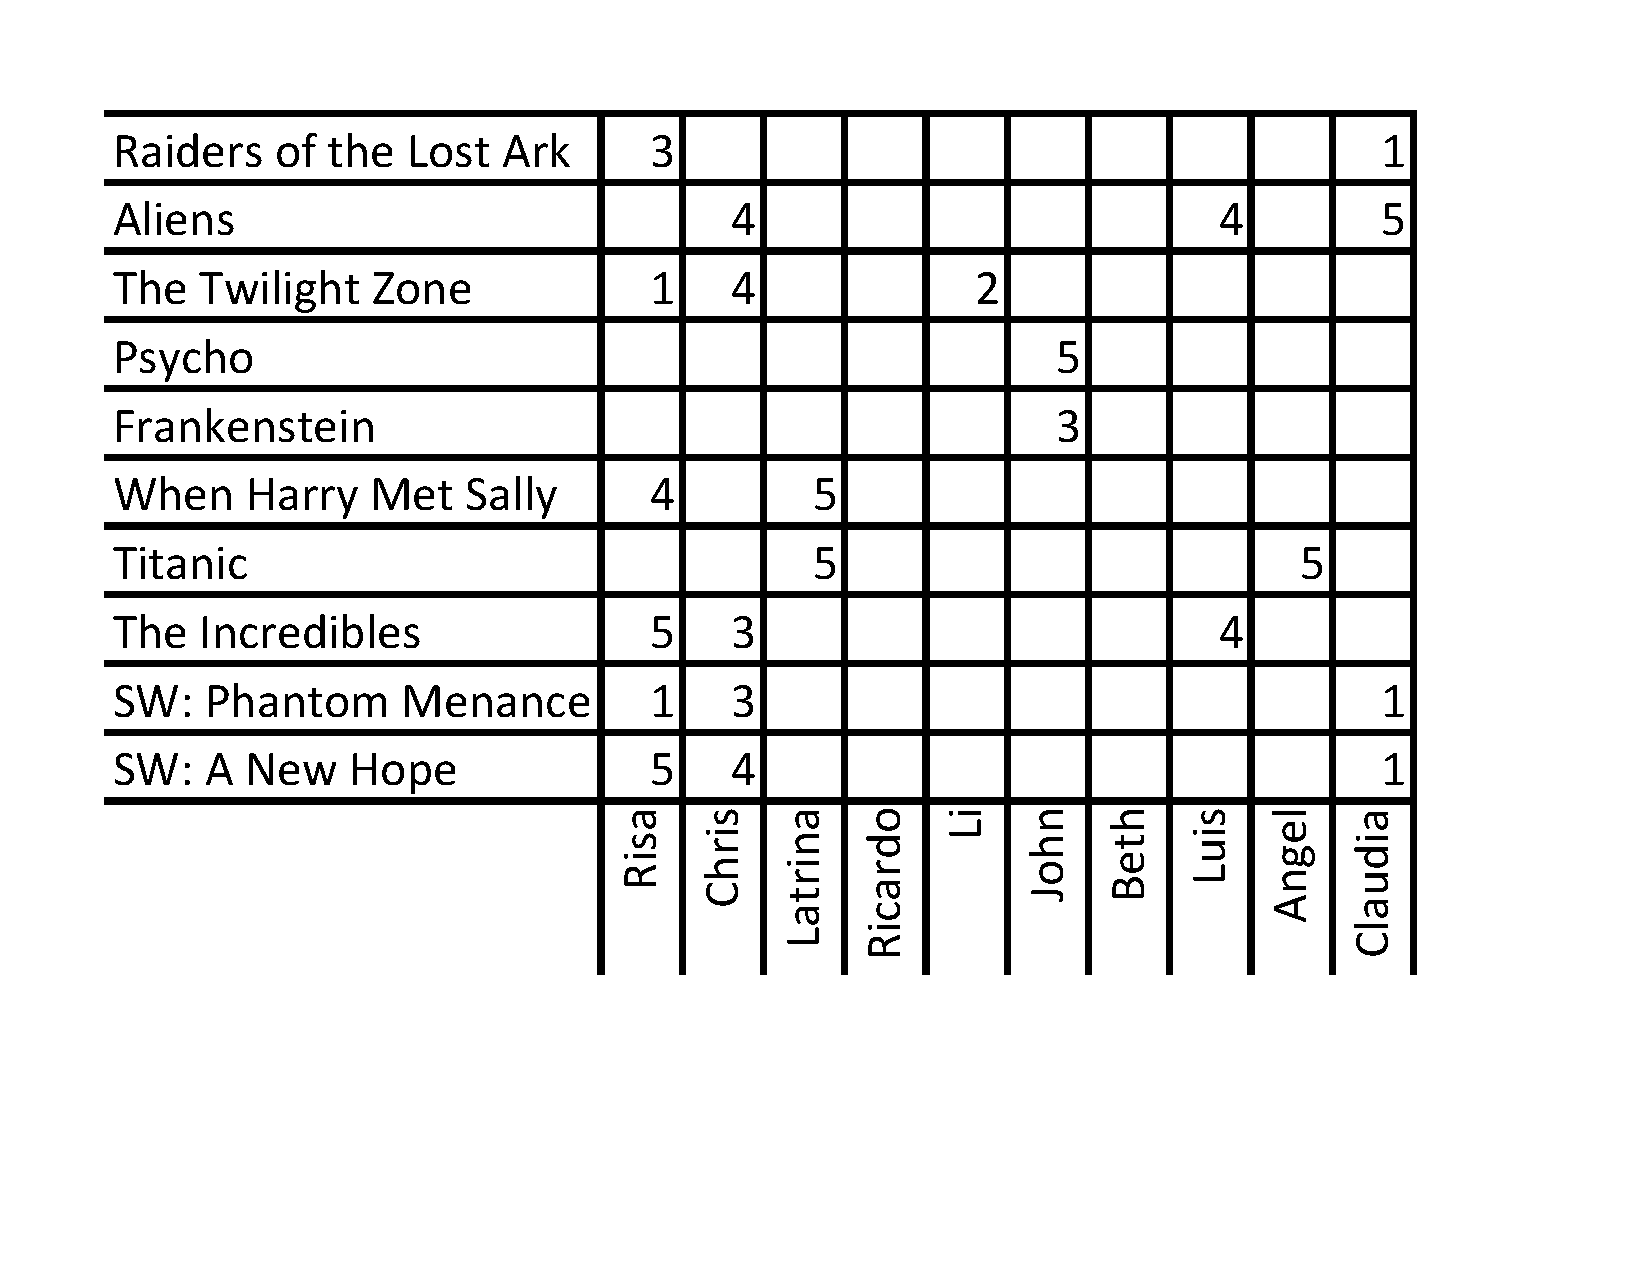
\includegraphics[width=1\textwidth]{lectUL/movieGrid} 
 \end{column}
 \end{columns}

\end{frame}
%***********************************************************
\begin{frame}{Classic Example: NNMF}

\begin{columns}
\begin{column}{0.5\textwidth}
\begin{itemize}
\item NonNegative Matrix Factorization
\item Motivation:
\begin{itemize}
\item Have a 2-D table
\item Entries in table describe outcome of interaction
\item Example: Netflix challenge
\item Want to recommend movies a user will like
\item This is \textbf{NOT} supervised learning
\item We do this by mapping into a latent space
\end{itemize}
\end{itemize}
 \end{column}
\begin{column}{0.5\textwidth}
    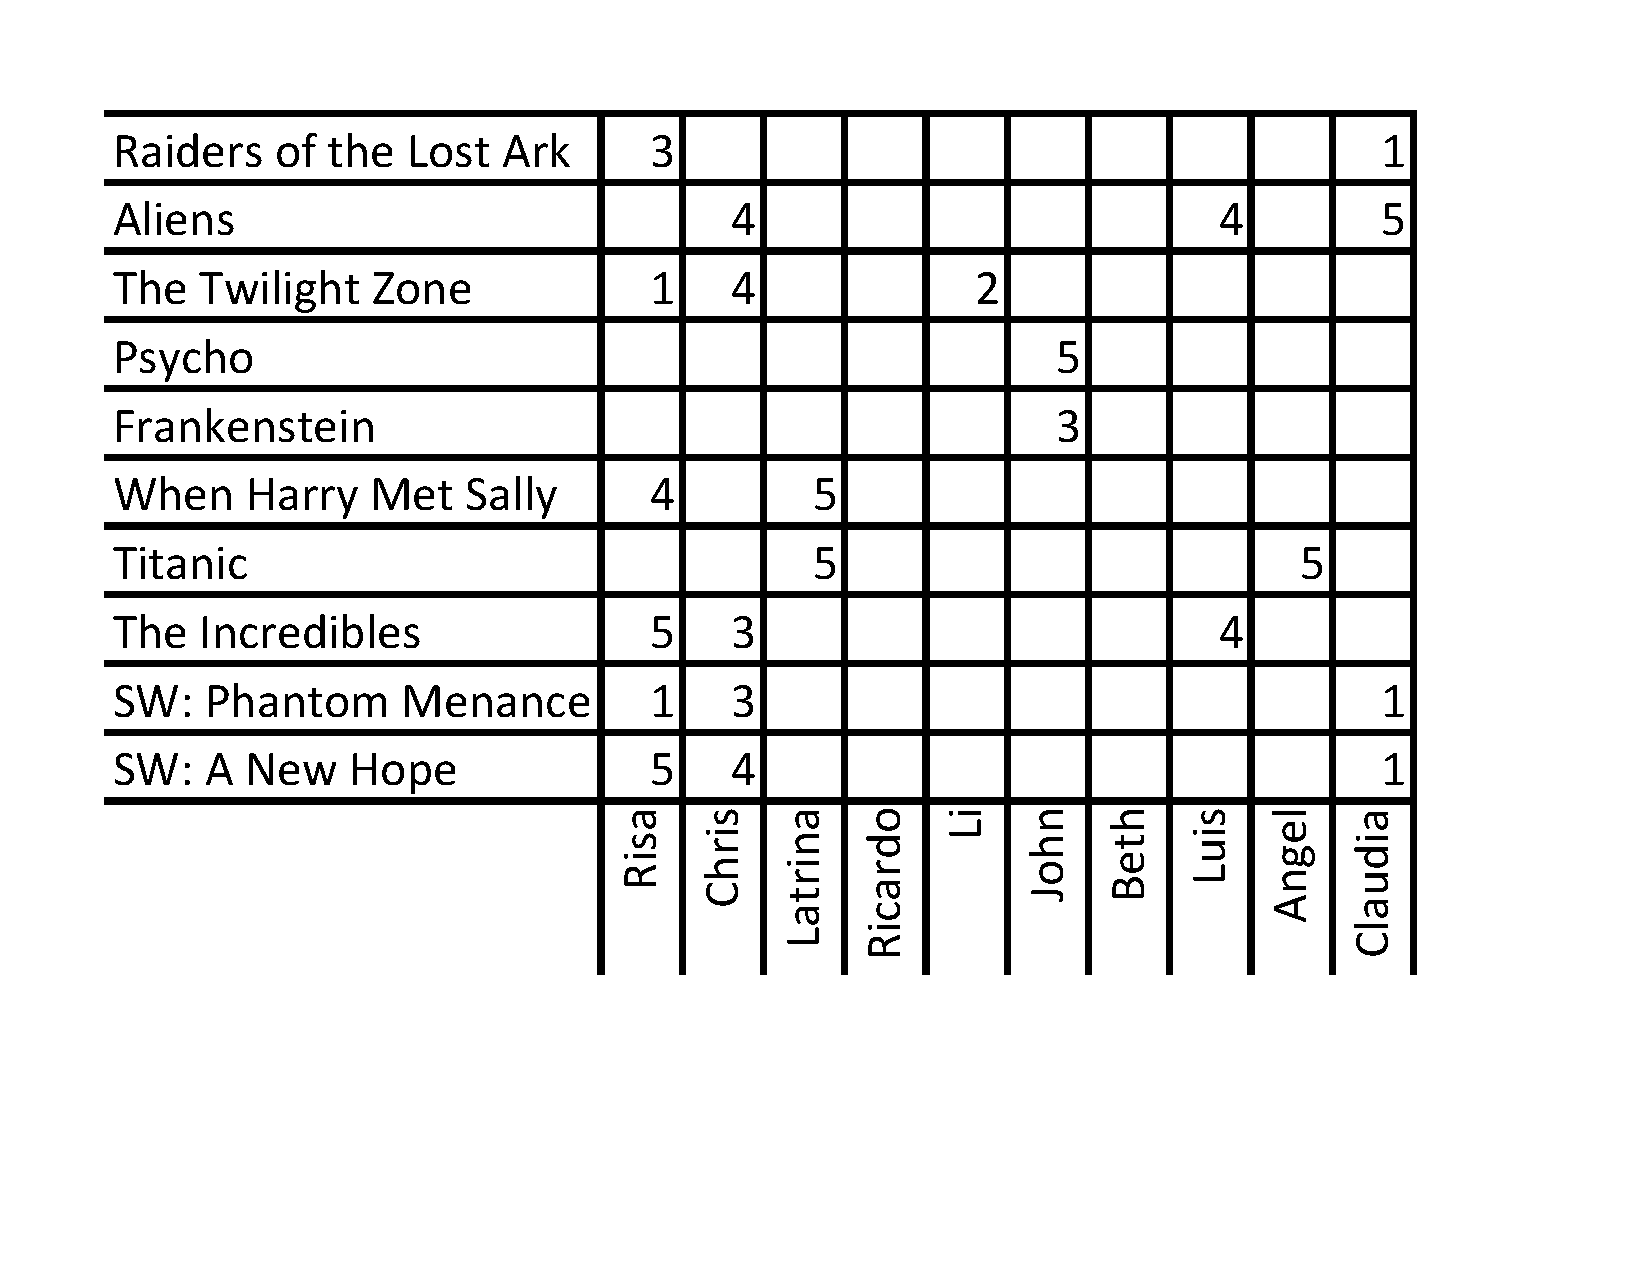
\includegraphics[width=1\textwidth]{lectUL/movieGrid} 
 \end{column}
 \end{columns}

\end{frame}
%***********************************************************
\begin{frame}{Movie-User Latent Space}
% http://www.quuxlabs.com/blog/2010/09/matrix-factorization-a-simple-tutorial-and-implementation-in-python/
\begin{itemize}
\item Assume there is some latent feature(s) that specify a user's rating
\begin{itemize}
\item Could be the stars
\item Could be the genre
\item Could be the era
\item $\ldots$
\end{itemize}
\item Assume that the number of latent features is $\ll$ the size of the rating matrix
\end{itemize}

\end{frame}
%***********************************************************
\begin{frame}{Classic Example: NNMF}

\begin{itemize}
\item Motivation:
\begin{itemize}
\item Have a 2-D table
\item Entries in table describe outcome of interaction
\item Example: Netflix challenge
\end{itemize}
\item We have a bunch of (movie, user, score) triples
\item Stored in an $n$ by $m$ matrix $V$ ($n$ movies, $m$ users)
\begin{itemize}
	\item Idea: map $i$th movie to a latent $k$-dimensional point $m_i$
	\item And map $j$th user to a latent $k$-dimensional point $u_j$
	\item Such that the score user $i$ gives to movie $j$ $\approx m_i \cdot u_j$
	\item Higher scores indicate higher rating
\end{itemize}
\item Many formulations; one is:
	$$ \min_{\{m_1, m_2, ..., u_1, u_2, ...\}} \sum_{i, j} (V_{i,j} - m_i \cdot u_j)^2$$
\end{itemize}

\end{frame}
%***********************************************************

\begin{frame}{Classic Example: NNMF}

\begin{itemize}
\item Many formulations; one is:
	$$ \min_{\{m_1, m_2, ..., u_1, u_2, ...\}} \sum_{i, j} (V_{i,j} - m_i \cdot u_j)^2$$
\end{itemize}
	\begin{itemize}
	\item Where $m_i$  and $u_j$ are the latent movie and user positions
	\item This is basically an optimization problem
	\item Where we are minimizing the loss of the squared error
	\item Can be solved many ways, including gradient descent % another approach is alternating least squares: Fix the user, solve for movies, then flip: fix the movies, solve for users
	\item ``Non-negative'' since often we want all latent vectors to be positive
	\item Turns out that the latent space is often meaningful!
	\end{itemize}
\end{frame}

%***********************************************************
\begin{frame}{Data Tend to Cluster}

\begin{columns}
\begin{column}{0.7\textwidth}
\begin{itemize}
	\item Ex: users score movies on 0-5 scale
	\item Imagine mapping movies, users to 2-D latent space
	\begin{itemize} 
	\item Imagine Action movies map near to $\langle 0, 2.5 \rangle$
	\item Rom Coms near to $\langle 2.5, 0 \rangle$
	\end{itemize}
	\item Then users will cluster according to prefs.  Why?
	\begin{itemize} 
	\item If I like only Action, I map close to $\langle 0, 2 \rangle$... since $\langle 0, 2.5 \rangle \cdot
		\langle 0, 2 \rangle = 5$ rating
	\item So people who like only Action cluster around $\langle 0, 2.5 \rangle$
	\item If I like only Rom Coms, I map close to $\langle 2, 0 \rangle$... since $\langle 2.5, 0 \rangle \cdot
		\langle 2, 2 \rangle = 5$ rating
	\item So people who like Rom Coms cluster around $\langle 0, 2.5 \rangle$
	\item If I like both, map to $\langle 2, 2 \rangle$... will give me $5$ rating for both
	\item So people who like both cluster around $\langle 2.5, 2.5 \rangle$
	\end{itemize}
\end{itemize}	
\end{column}
\begin{column}{0.3\textwidth}
    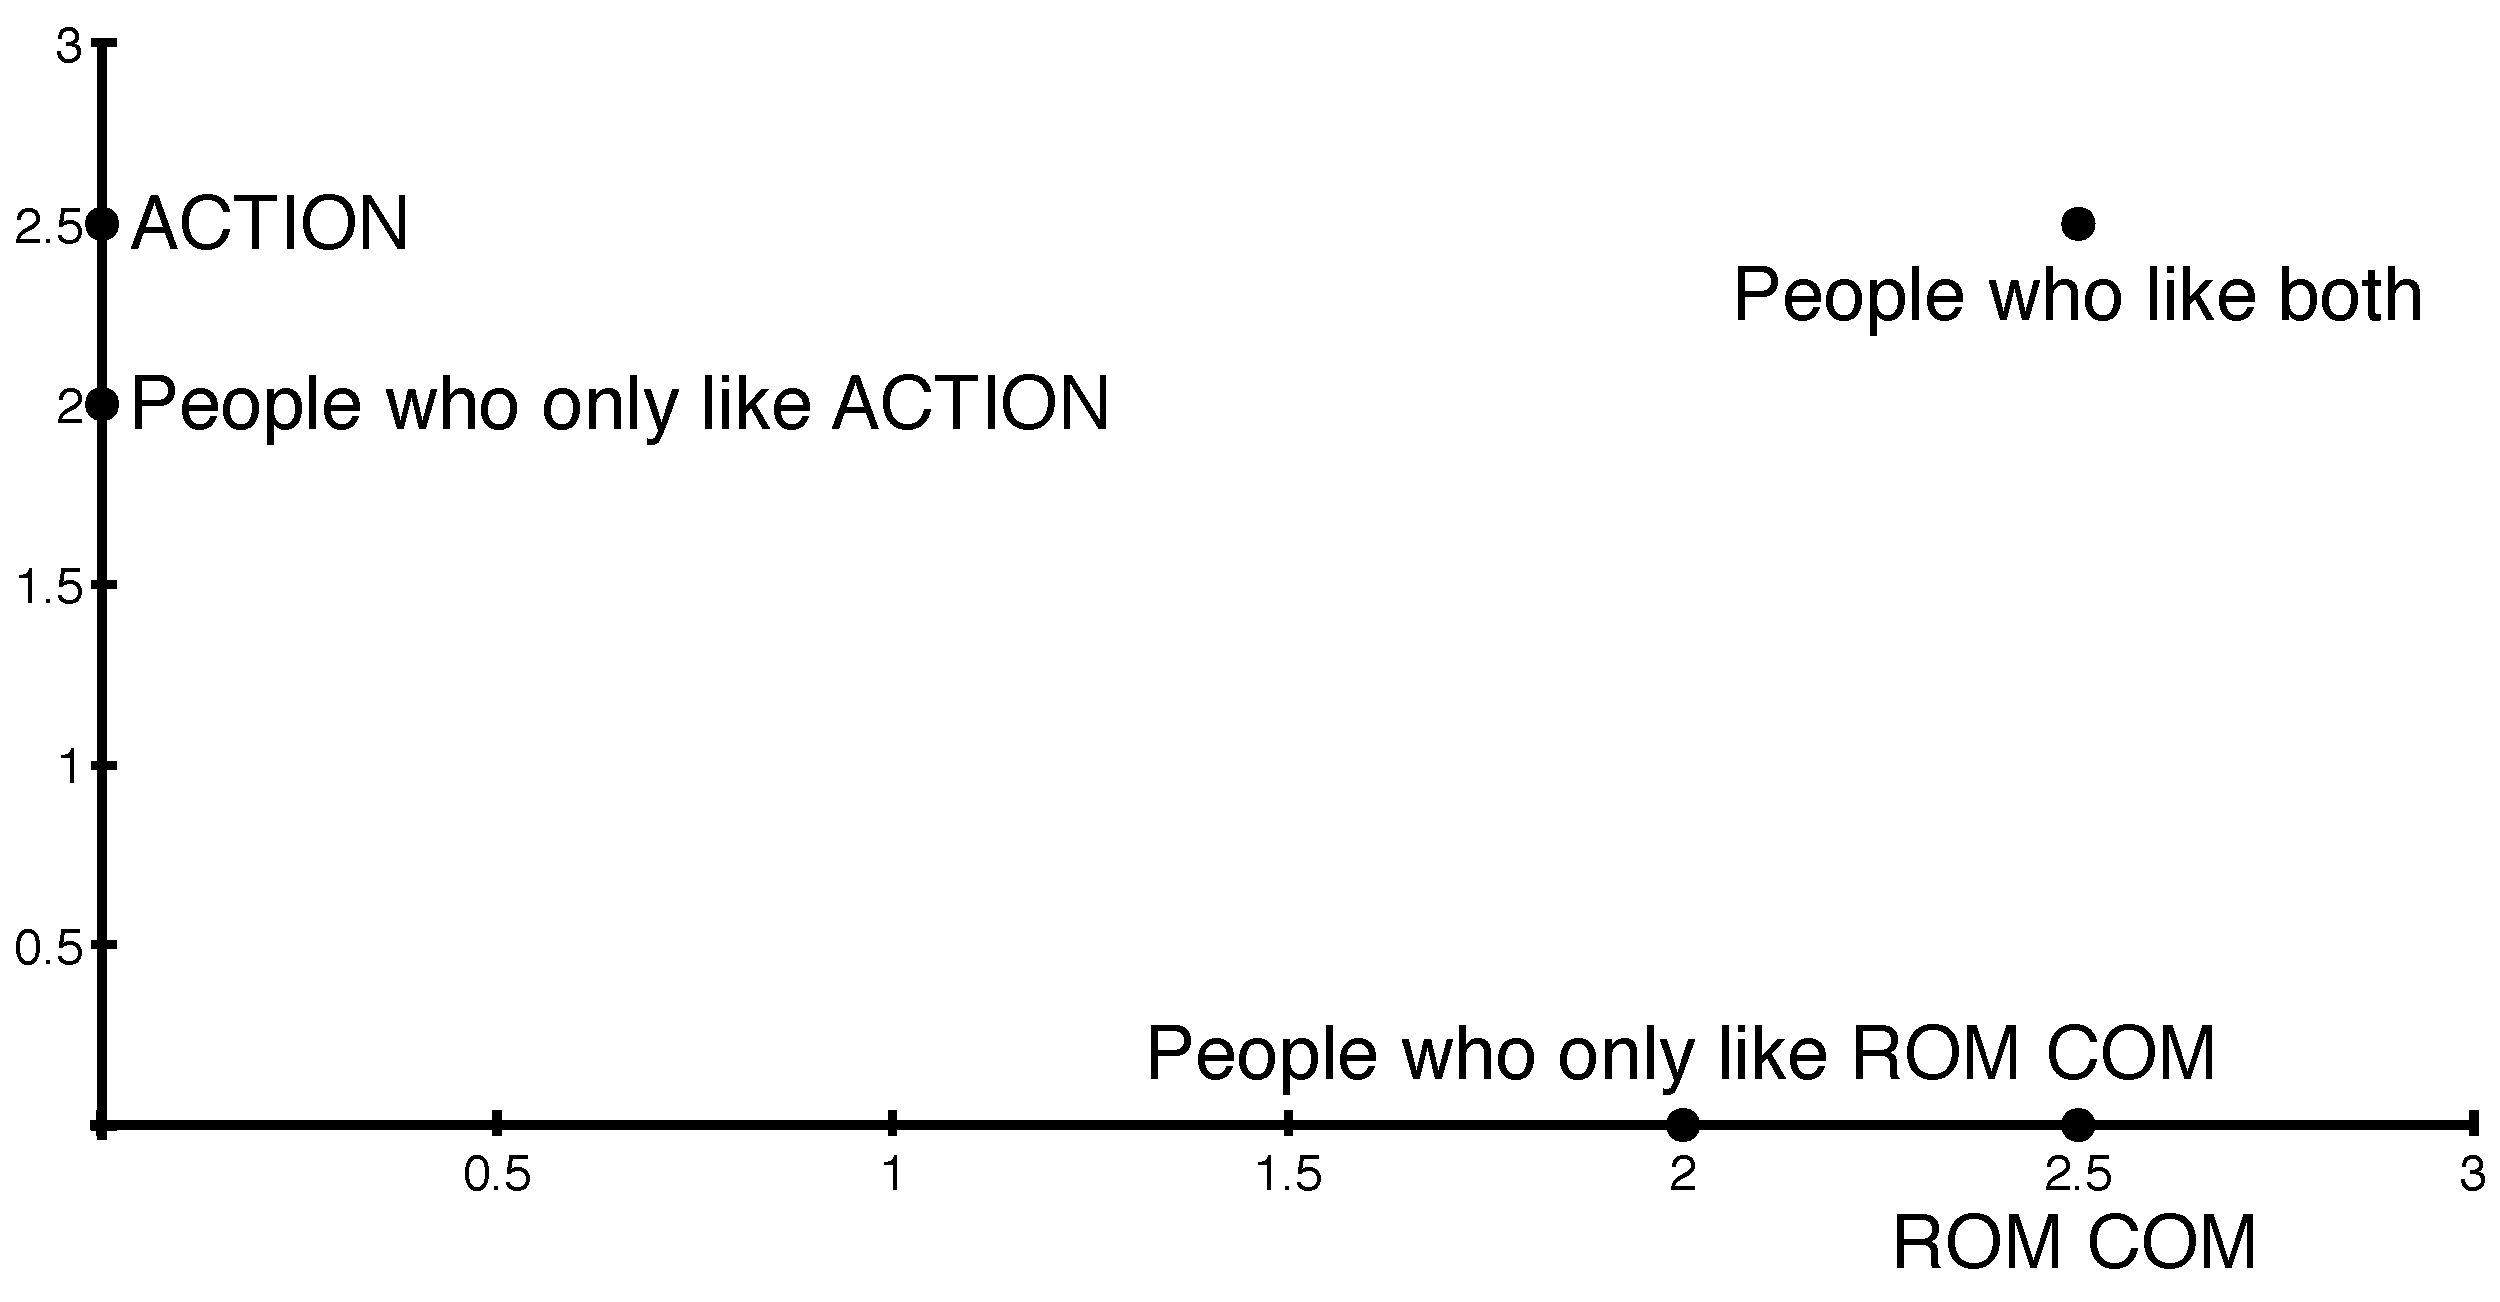
\includegraphics[width=1\textwidth]{lectUL/movieLatentSpace.pdf} 
\end{column}
\end{columns}
	
\end{frame}

%***********************************************************
\begin{frame}{Why Called ``Matrix Factorization''?}

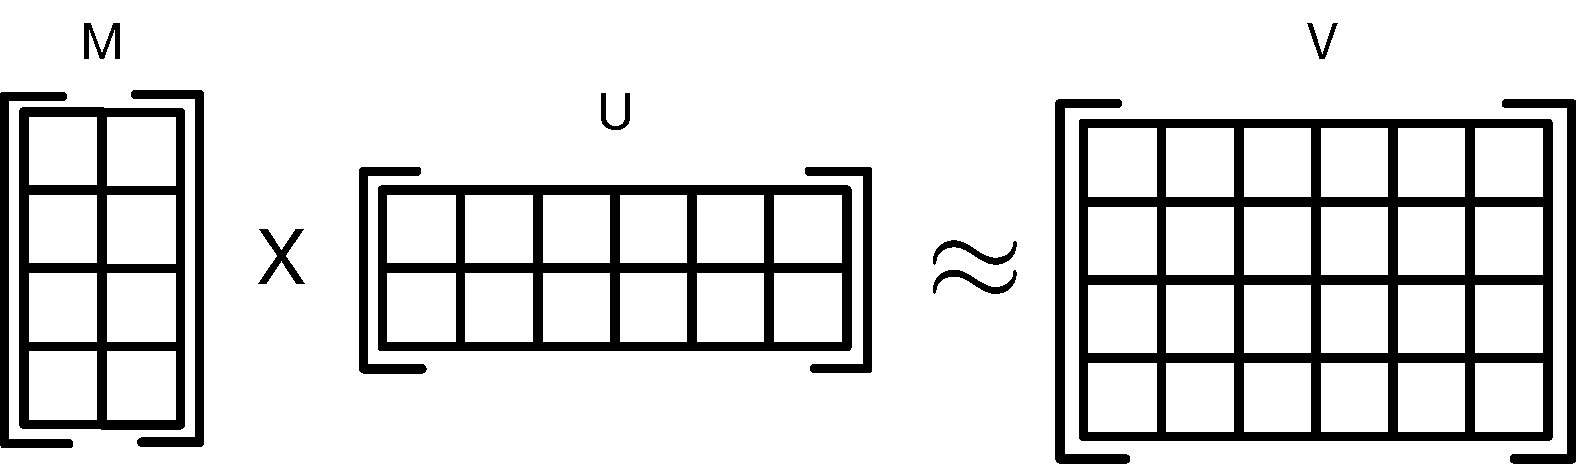
\includegraphics[width=0.9\textwidth]{./lectUL/matrixFactorization.pdf}

\begin{itemize}
\item View $M$ matrix as latent positions of movies
\item View $U$ matrix as latent positions of users
\item We are trying to learn $M$, $U$ from $V$
\end{itemize}

\end{frame}
%***********************************************************
\begin{frame}{Closing Comments}

\begin{itemize}
\item ``Supervised'' vs. ``Unsupervised'' distinction not always hard
\item ``Clustering'' vs. ``Latent Variable'' distinction not always hard
\begin{itemize}
	\item All but the most ad-hoc clustering algorithms can be written as latent variable problems
	\item Example: NNMF is unsupervised
\begin{itemize}
\item There's no ``Rom-com'' label
\item But it is a predictive model for scores
\item Once you map the user and movies, you can get a score indicating if someone will like a movie
\end{itemize}
\end{itemize}
\end{itemize}
	
\end{frame}
%***********************************************************
\begin{frame}{Questions?}
\begin{itemize}
	\item What do we know now that we didn't know before?
	\begin{itemize}
		\item We know what unsupervised learning is
		\item We know some techniques for clustering data 
		\item We have seen some variations on how to cluster
		\item We know about the Netflix challenge
	\end{itemize}
	\item How can we use what we learned today?
	\begin{itemize}
		\item We can try clustering data!
	\end{itemize}
\end{itemize}
\end{frame}

\end{document}
